\section{Polysemous words prediction}
\label{sec:polysemous-words-prediction}
In this section, we look at various methods for predicting whether or not a word is polysemous. First, we will apply methods from topological data analysis to word embeddings. In particular, we will investigate the notion of topological polysemy in \cref{sec:analysis-of-embeddings-topological-polysemy} and geometric anomaly detection in \cref{sec:analysis-of-embeddings-geometric-anomaly-detection}. We use topological polysemy to estimate the number of meanings of a word, given its word vector. Particularly, we would like to see if the $\text{TPS}_n(w)$ score measures polysemy. In addition to this, we would like to see if singular word vectors as identified by geometric anomaly detection are polysemous. Following, we will compute the estimated intrinsic dimension of word embeddings and compare the results with the number of word meanings in \cref{sec:analysis-of-embeddings-intrinsic-dimension-estimation}. Finally, we end the section by proposing supervised models to predict the number of word meanings in \cref{sec:analysis-of-embeddings-supervised-polysemy-prediction}.

\subsection{Topological polysemy}
\label{sec:analysis-of-embeddings-topological-polysemy}
In this subsection, we will apply topological polysemy (\cref{sec:topological-polysemy}) to the word embeddings from the SGNS-enwiki model. Additionally, we will also train another word2vec model using the same training data used by \cite{jakubowski2020topology} and apply topological polysemy to its word embeddings. We refer to this word2vec model as the \textit{SGNS-semeval} model. Furthermore, we will compare the results to topological polysemy applied to word embeddings from pre-trained models, namely the fastText model (\textit{fastText.TPS.300d}) used in experiments of \cite{jakubowski2020topology}, the \textit{GoogleNews-vectors-negative300} (shortened to \textit{GoogleNews300}) word embeddings from \cite{GoogleCodeArchiveWord2vec}, the \textit{glove.840B.300d} word embeddings from \cite{GloVeProject2014} and the English (\textit{fastText.en.300d}) word embeddings from \cite{grave2018learning}. The fastText.TPS.300d model was kindly given in private communication with one of the authors of topological polysemy \cite{ZibrowiusPrivComs2021}.

The authors of topological polysemy, \cite{jakubowski2020topology}, trained a fastText model on training data from the \textit{SemEval-2010 Task 14: Evaluation Setting for Word Sense Induction \& Disambiguation Systems} \cite{manandhar-klapaftis-2009-semeval}. The training data from the SemEval task consists of several sentences related to 100 polysemous words (50 nouns and 50 verbs). The SemEval data set also includes the number of true meanings (also called \textit{gold standard} or \textit{GS}) for each of the 100 polysemous words, as perceived by humans. In private communication with one of the authors of the topological polysemy measure \cite{ZibrowiusPrivComs2021}, we received some additional information regarding their training and data preprocessing choices. In particular, they stated that they used a fastText model with vector dimensionality of 300, that they removed all punctuation from words and replaced capital letters with the corresponding small letters. To compare with the $\text{TPS}_n(w)$, the authors use the 100 polysemous words, words from the SemEval training data that has a \textit{WordNet} \cite{fellbaum1998} entry and all words in SemEval training data. WordNet is a lexical database of the English language. In particular, it allows for querying nearly any word from the English language and returns the \textit{synsets} of the word. The synset of a word $w$ is a word that shares a similar meaning to the word $w$. In other words, by querying a word in WordNet, we can get the number of meanings of a word, as perceived by WordNet. Furthermore, the Pearson correlation coefficient \cite{James2013} is computed between $\text{TPS}_n(w)$ and GS, the number of synsets for WordNet words and the word frequency as they appear in the SemEval training data, respectively. \cite{jakubowski2020topology} shows that there is a moderate (positive) correlation between $\text{TPS}_n(w)$ and GS at $n \in \enclc{40, 50, 60}$, a decreasing correlation between $\text{TPS}_n(w)$ and the number of synsets for WordNet words and no correlation between $\text{TPS}_n(w)$ and word frequencies.

Furthermore, we will describe how we applied topological polysemy to our word embeddings. We first implemented topological polysemy using the steps we described in \cref{sec:topological-polysemy}, utilizing multiprocessing and the ScaNN \cite{scann2020} approximate nearest neighbour algorithm to speed up the computation. We chose ScaNN because it performs well when applied to word embeddings, as shown in \cite{AnnBenchmarks2021}. We used the \path{ripser} \cite{ctralie2018ripser} Python package to compute Vietoris–Rips complexes. Next, we trained the SGNS-semeval model using the training data from the SemEval task and the hyperparameters used to train the SGNS-enwiki model from \cref{sec:word2vec-hyperparameter-choices}. From the training of SGNS-semeval, we got a vocabulary of size $\sim$122K words and a corpus of size $\sim$67 million. Following, we will compare the results from the experiments of \cite{jakubowski2020topology} by computing topological polysemy at varying levels of $n$ using the word embeddings of SGNS-enwiki and SGNS-semeval. Finally, we compare the results using the SGNS-enwiki and SGNS-semeval word embeddings to the word embeddings of the fastText.TPS.300d, GoogleNews300, glove.840B.300d and fastText.en.300d models.

We computed topological polysemy at varying levels of $n$ using the word embeddings of the SGNS-enwiki and SGNS-semeval models, and show the results in \cref{table:tps-n-correlation-sgns-enwiki,table:tps-n-correlation-sgns-semeval}. In \cref{table:tps-n-correlation-sgns-enwiki}, we see that the correlation between $\text{TPS}_n$ and GS is rather stable with respect to $n$. In particular, we notice that the correlation between $\text{TPS}_n$ and GS is negative, suggesting a relationship in the opposite direction of the results from \cite[Table 1]{jakubowski2020topology}. Nonetheless, we see a decreasing correlation when comparing $\text{TPS}_n$ versus the number of WordNet synsets for each word, and a negligible correlation between $\text{TPS}_n$ and word frequencies of the top 10000 most common words. Furthermore, in \cref{table:tps-n-correlation-sgns-semeval}, we observe a decreasing negative correlation going towards zero between $\text{TPS}_n$ and GS, meaning that the SGNS-semeval model performs worse than the SGNS-enwiki model on this particular task. This result indicates that by training SGNS-semeval on a smaller vocabulary than the vocabulary of SGNS-enwiki, we get worse results. Furthermore, we see a decreasing correlation between $\text{TPS}_n$ and the number of WordNet synsets and a negligible correlation between $\text{TPS}_n$ and word frequencies of the top 10000 most common words. Although the negative correlation between $\text{TPS}_n$ and the number of WordNet synsets is larger for the SGNS-semeval model than the SGNS-enwiki model, it is still not particularly large. In addition to this, we are considering a lot fewer words when computing the correlation in the SGNS-semeval model than the SGNS-enwiki model (see sample size).
\begin{table}[H]
    \centering
    \begin{tabular}{@{}rrrr@{}}
    \toprule
    $n$ & $\text{TPS}_n$ vs. GS & $\text{TPS}_n$ vs. synsets & $\text{TPS}_n$ vs. frequency \\
    \midrule
    \trcolor 10  & -0.353        & -0.077             & \textbf{-0.043}               \\
    40  & \textbf{-0.383}        & -0.181             & -0.041               \\
    \trcolor 50  & -0.380        & -0.190             & -0.041               \\
    60  & -0.381        & -0.196             & -0.040               \\
    \trcolor 100 & -0.380        & \textbf{-0.205}             & -0.033               \\
    \midrule
    \textit{sample size} & 98 & 144 412 & 10 000 \\
    \bottomrule
    \end{tabular}
    \caption{Correlations between $\text{TPS}_n$ and the number of word meanings as perceived by humans (GS), the number of WordNet synsets and the word frequencies of the top 10000 most common words from the SGNS-enwiki model. \textbf{Bold} values indicate the largest (absolute) correlation.}
    \label{table:tps-n-correlation-sgns-enwiki}
\end{table}
\begin{table}[H]
    \centering
    \begin{tabular}{@{}rrrr@{}}
    \toprule
    $n$ & $\text{TPS}_n$ vs. GS & $\text{TPS}_n$ vs. synsets & $\text{TPS}_n$ vs. frequency \\
    \midrule
    \trcolor 10  & \textbf{-0.300}        & -0.248             & 0.102                \\
    40  & -0.201        & -0.300             & \textbf{0.120}                \\
    \trcolor 50  & -0.194        & -0.304             & 0.116                \\
    60  & -0.169        & -0.306             & 0.110                \\
    \trcolor 100 & -0.130        & \textbf{-0.310}             & 0.098                \\
    \midrule
    \textit{sample size} & 100 & 62 111 & 10 000 \\
    \bottomrule
    \end{tabular}
    \caption{Correlations between $\text{TPS}_n$ and the number of word meanings as perceived by humans (GS), the number of WordNet synsets and the word frequencies of the top 10000 most common words from the SGNS-semeval model. \textbf{Bold} values indicate the largest (absolute) correlation.}
    \label{table:tps-n-correlation-sgns-semeval}
\end{table}

To further broaden our understanding of the results we got from computing topological polysemy of the word embeddings of the SGNS-enwiki and the SGNS-semeval models, we plot $\text{TPS}_n(w)$ against the GS, the number of WordNet synsets and word frequencies. We visualize the results in \cref{fig:tps-n-correlation-sgns-enwiki,fig:tps-n-correlation-sgns-semeval}, and for each plot, we let $n$ be equal to the most optimal value for each column in \cref{table:tps-n-correlation-sgns-enwiki,table:tps-n-correlation-sgns-semeval}. In \cref{fig:tps-n-correlation-sgns-enwiki}, we see a similar situation to the results from \cite[Figures 8 and 9]{jakubowski2020topology}, namely that we see an indication of a linear relationship between $\text{TPS}_n(w)$ and the SemEval gold standard and that we see a clear trend between $\text{TPS}_n(w)$ and the number of synsets in WordNet. In \cref{fig:tps-n-correlation-sgns-enwiki} (c) it is clear that there is no apparent relationship between $\text{TPS}_n(w)$ and the word frequencies. Following, we see a similar situation appearing in \cref{fig:tps-n-correlation-sgns-semeval}. These results suggest that, by computing $\text{TPS}_n(w)$ of the SGNS-enwiki word embeddings, which has a vocabulary much larger than in the experiments of \cite{jakubowski2020topology}, we are unable to use $\text{TPS}_n(w)$ alone for predicting the number of word meanings, as given by the number of WordNet synsets.
\begin{figure}[H]
    \centering
    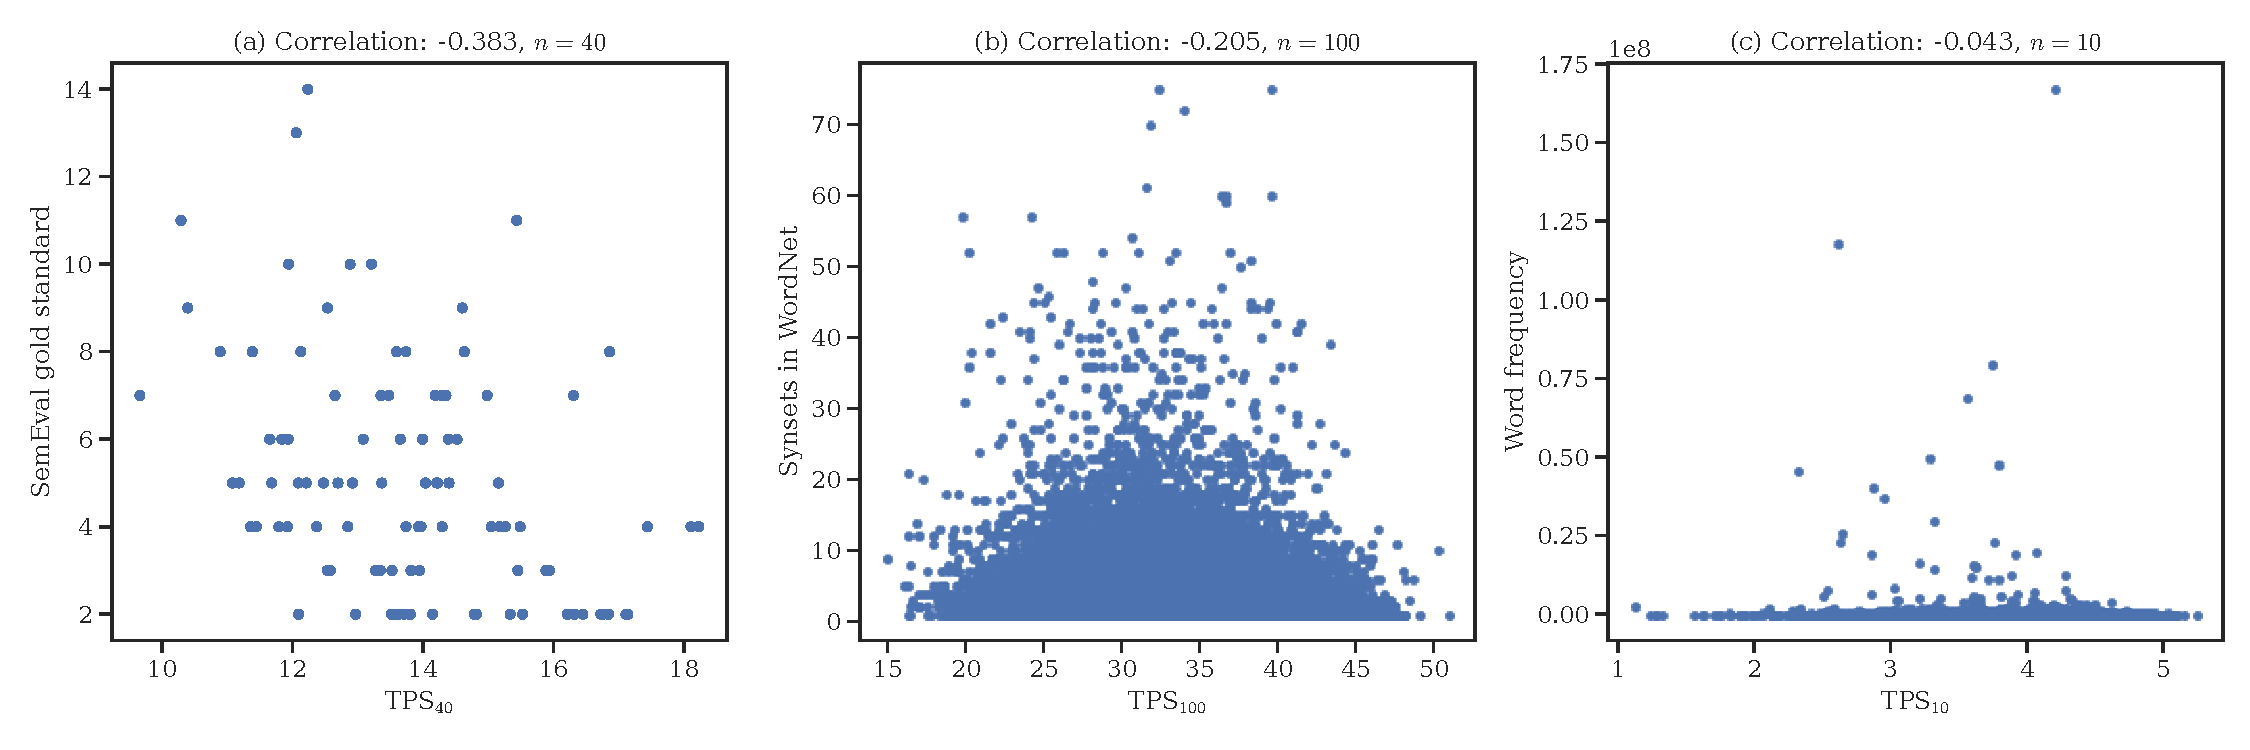
\includegraphics[width=\textwidth]{thesis/figures/tps-n-correlation-sgns-enwiki.pdf}
    \caption{Topological polysemy $\text{TPS}_n(w)$ of the word embeddings of SGNS-enwiki plotted against the GS (a), the number of WordNet synsets (b) and word frequencies (c). Plots are inspired by \cite[Figures 8 and 9]{jakubowski2020topology}.}
    \label{fig:tps-n-correlation-sgns-enwiki}
\end{figure}
\begin{figure}[H]
    \centering
    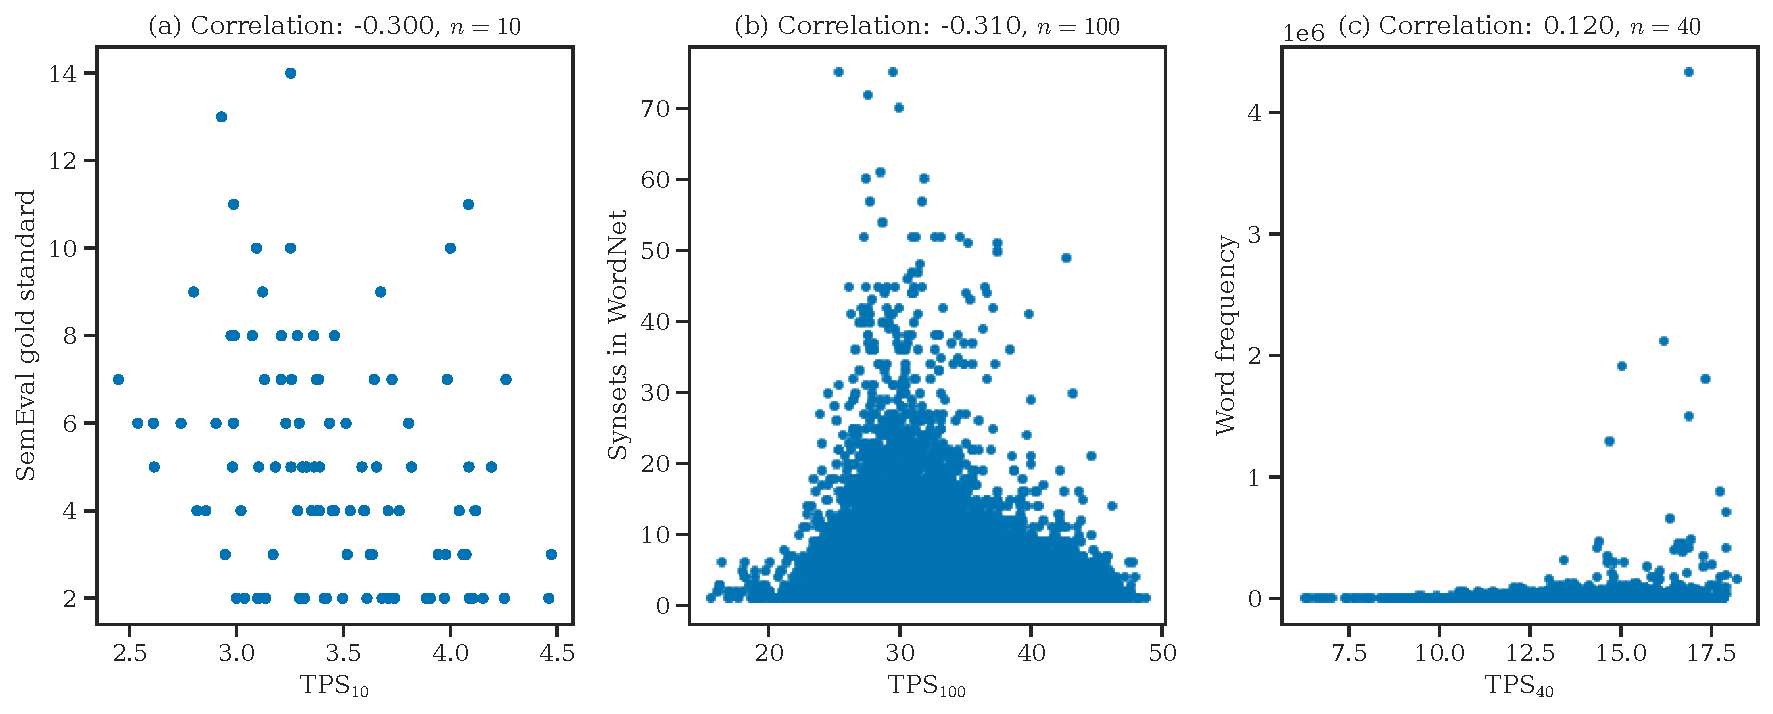
\includegraphics[width=\textwidth]{thesis/figures/tps-n-correlation-sgns-semeval_2010_task_14.pdf}
    \caption{Topological polysemy $\text{TPS}_n(w)$ of the word embeddings of SGNS-semeval plotted against the GS (a), the number of WordNet synsets (b) and word frequencies (c). Plots are inspired by \cite[Figures 8 and 9]{jakubowski2020topology}.}
    \label{fig:tps-n-correlation-sgns-semeval}
\end{figure}

Following, we compared the results of computing $\text{TPS}_n(w)$ of the word embeddings of the SGNS-enwiki and SGNS-semeval models to the word embeddings of the fastText.TPS.300d, GoogleNews300, glove.840B.300d and fastText.en.300d models. We show the $\text{TPS}_n(w)$ results of using the fastText.TPS.300d model in \cref{table:tps-n-correlation-fasttext-tps-word-embeddings}, and using the GoogleNews300, glove.840B.300d and fastText.en.300d in \cref{table:tps-n-correlation-external-word-embeddings}. We did not compute the correlation between $\text{TPS}_n(w)$ and word frequencies in \cref{table:tps-n-correlation-fasttext-tps-word-embeddings,table:tps-n-correlation-external-word-embeddings}, since we did nott have the data available. In addition to this, it is unlikely that $\text{TPS}_n(w)$ and word frequencies have anything in common, as shown in the previous results using the SGNS-enwiki and SGNS-semeval models, as well as by the experiments of \cite{jakubowski2020topology}.

\begin{table}[H]
    \centering
    \begin{tabular}{@{}rrr@{}}
    \toprule
    $n$ & $\text{TPS}_n$ vs. GS & $\text{TPS}_n$ vs. synsets \\
    \midrule
    \trcolor 10 & 0.131	& \textbf{0.135} \\
    40 & 0.395 & 0.066 \\
    \trcolor 50 & \textbf{0.416} & 0.053 \\
    60 & 0.363 & 0.043 \\
    \trcolor 100 & 0.301 & 0.020 \\
    \midrule
    \textit{sample size} & 100 & 62 049 \\
    \bottomrule
    \end{tabular}
    \caption{Correlations between $\text{TPS}_n$ and the number of word meanings as perceived by humans (GS) and the number of WordNet synsets from the fastText.TPS.300d model. \textbf{Bold} values indicate the largest (absolute) correlation.}
    \label{table:tps-n-correlation-fasttext-tps-word-embeddings}
\end{table}
In \cref{table:tps-n-correlation-fasttext-tps-word-embeddings}, we see similar results to the experiments of \cite{jakubowski2020topology}, namely that we get a modest, positive correlation when comparing $\text{TPS}_n(w)$ to the SemEval gold standard, and that we get a decreasing correlation when comparing $\text{TPS}_n(w)$ to the number of WordNet synsets. We note, however, that we did not get exactly the same correlation results as \cite{jakubowski2020topology}, which could be affected by the use of ScaNN, which approximates the nearest neighbours of words.

\begin{table}[H]
    \centering
    \begin{tabular}{ccccccc}
    \toprule
    \multicolumn{1}{c}{\multirow{2}{*}{$n$}} & \multicolumn{2}{c}{GoogleNews300}    & \multicolumn{2}{c}{glove.840B.300d}              & \multicolumn{2}{c}{fastText.en.300d}             \\
    \cmidrule(l){2-7} 
    \multicolumn{1}{c}{}                   & \makecell[tc]{$\text{TPS}_n$ vs.\\GS} & \makecell[tc]{$\text{TPS}_n$ vs.\\synsets} & \makecell[tc]{$\text{TPS}_n$ vs.\\GS} & \makecell[tc]{$\text{TPS}_n$ vs.\\synsets} & \makecell[tc]{$\text{TPS}_n$ vs.\\GS} & \makecell[tc]{$\text{TPS}_n$ vs.\\synsets} \\ \midrule
    \trcolor 10           & \textbf{-0.446}  & -0.095       & -0.103  & 0.008        & -0.240  & \textbf{0.114}        \\
    40           & \textbf{-0.446}  & -0.166       & \textbf{-0.125}  & -0.039       & \textbf{-0.289}  & 0.110        \\
    \trcolor 50           & -0.436  & -0.174       & -0.053  & -0.044       & -0.199  & 0.108        \\
    60           & -0.428  & -0.180       & -0.023  & -0.048       & -0.150  & 0.105        \\
    \trcolor 100          & -0.417  & \textbf{-0.193}       & -0.053  & \textbf{-0.058}       & -0.105  & 0.099        \\
    \midrule
    \makecell[tc]{\textit{sample}\\\textit{size}} & 100 & 207 119 & 100 & 249 352 & 100 & 230 175 \\
    \bottomrule
    \end{tabular}
    \caption{Correlations between $\text{TPS}_n$ and the number of word meanings as perceived by humans (GS), and the number of WordNet synsets from the GoogleNews300, glove.840B.300d and fastText.en.300d models. \textbf{Bold} values indicate the largest (absolute) correlation.}
    \label{table:tps-n-correlation-external-word-embeddings}
\end{table}
Furthermore, in \cref{table:tps-n-correlation-external-word-embeddings} we see that the GoogleNews300 models yields particularly high values when comparing $\text{TPS}_n(w)$ to the SemEval gold standard, while the remaining models are modest at best. We also observe that when comparing $\text{TPS}_n(w)$ to the number of WordNet synsets, we do not get high correlation scores. These results further suggest that by only increasing the vocabulary of the word embedding model, we are not able to model the number of WordNet synsets efficiently, only using the $\text{TPS}_n(w)$ scores. Additionally, the correlation results shown in \cref{table:tps-n-correlation-external-word-embeddings} indicate that the $\text{TPS}_n(w)$ scores are behaving rather inconsistent across the data sets, and it is not clear if $\text{TPS}_n(w)$ measures polysemy of words.

To compare how well the various word embedding models agree on the $\text{TPS}_n(w)$, we created a correlation matrix comparing the $\text{TPS}_n(w)$ scores and the SemEval gold standard. Using a correlation matrix, we summarize the results nicely and further deepen our understanding of the results. By majority vote, we let $n=40$ when we compared the $\text{TPS}_n(w)$ scores to the SemEval gold standard. We show the correlation matrix in \cref{fig:correlation-matrix-tps-vs-gs}, where we see that the SGNS-enwiki, SGNS-semeval and GoogleNews300 models yield similar $\text{TPS}_{40}(w)$ scores. We also note that the fastText.TPS.300d model either yield no correlation or negative correlations when compared to the other models.
\begin{figure}[H]
    \centering
    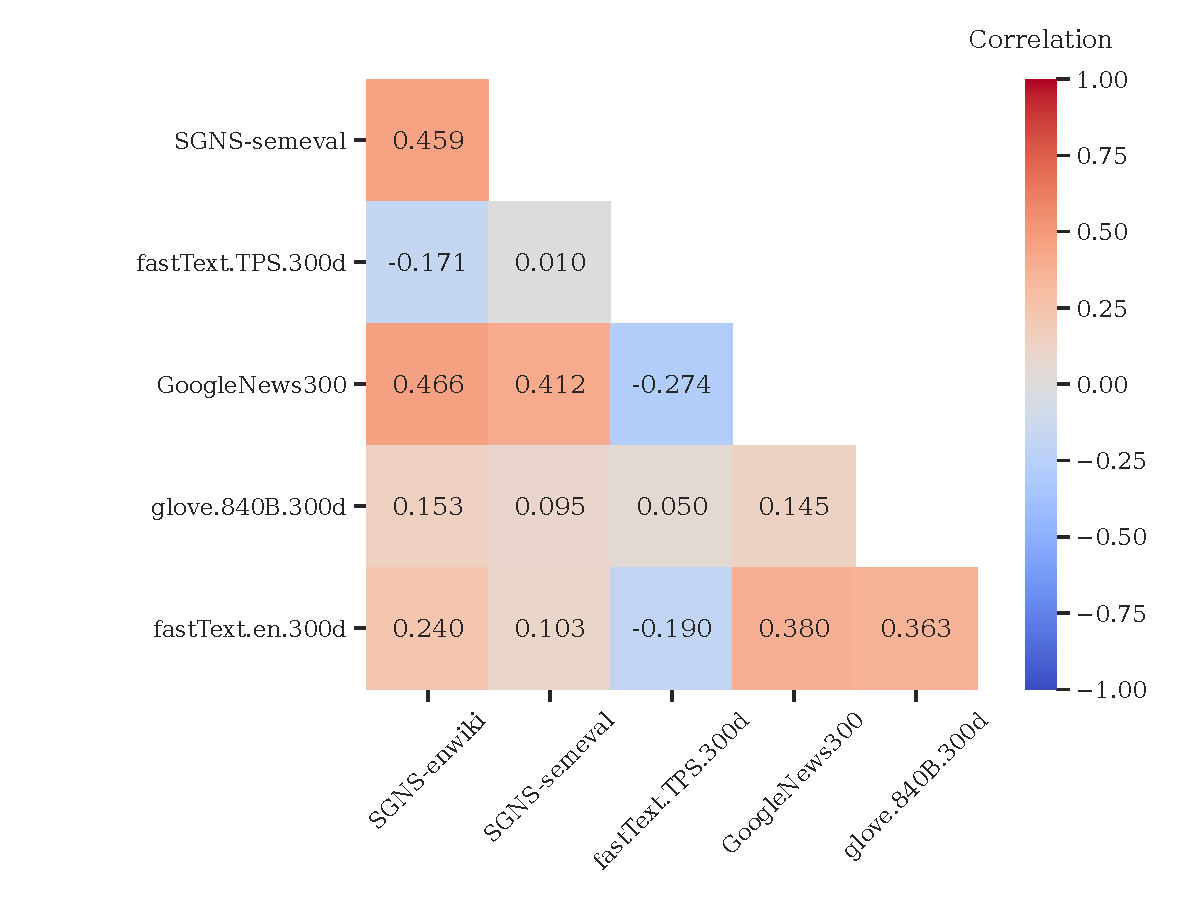
\includegraphics[width=0.8\textwidth]{thesis/figures/correlation-matrix-tps-vs-gs.pdf}
    \caption{Correlation matrix which compares word embedding models on correlations between the $\text{TPS}_{40}(w)$ scores and the SemEval gold standard. High (absolute) values indicate that the two models are similar in terms of scoring using $\text{TPS}_{40}(w)$.}
    \label{fig:correlation-matrix-tps-vs-gs}
\end{figure}

To deepen the understanding, we visualize the similarity of the SGNS-enwiki, SGNS-semeval and GoogleNews300 models in \cref{fig:tps-vs-gs-top-3-correlation-word-embedding-models}, where we can see linear relationships appearing. These results suggest that the SGNS-enwiki, SGNS-semeval and GoogleNews300 models agree on how to score using $\text{TPS}_{40}(w)$.
\begin{figure}[H]
    \centering
    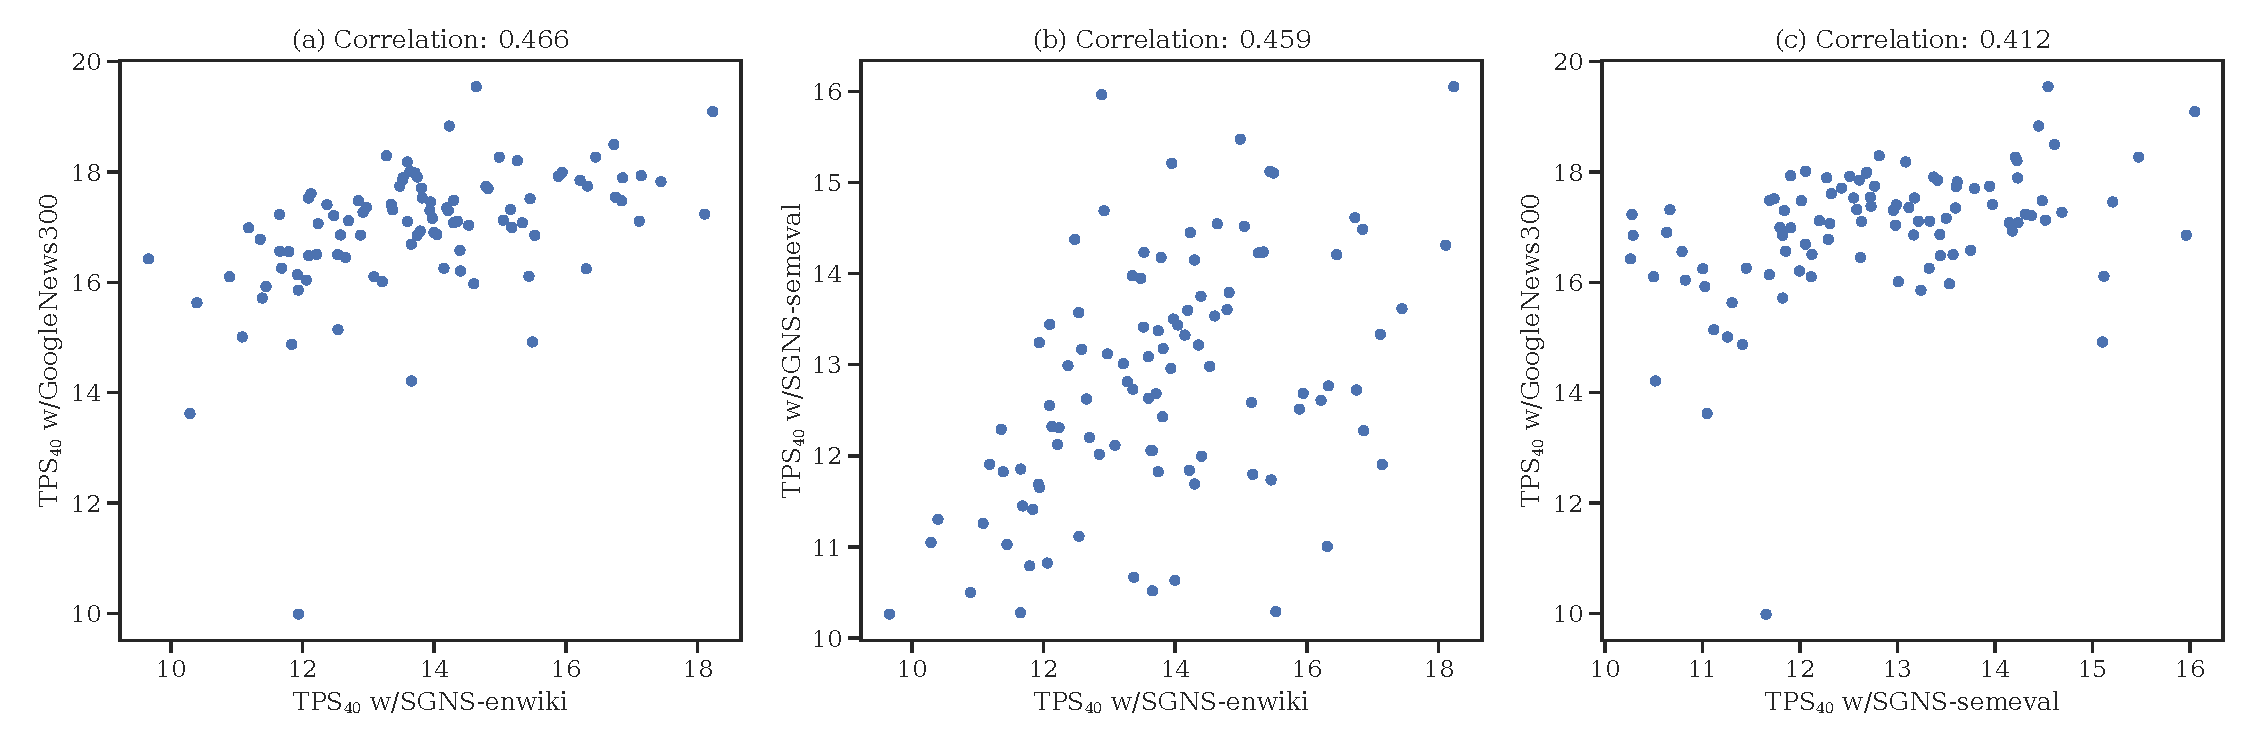
\includegraphics[width=\textwidth]{thesis/figures/tps-vs-gs-top-3-correlation-word-embedding-models.pdf}
    \caption{$\text{TPS}_{40}(w)$ scores plotted against each other using the SGNS-enwiki, SGNS-semeval and GoogleNews300 models.}
    \label{fig:tps-vs-gs-top-3-correlation-word-embedding-models}
\end{figure}

Following, we looked at the three negative correlations which we show in \cref{fig:correlation-matrix-tps-vs-gs} and visualize the negative relationships in \cref{fig:tps-vs-gs-top-3-negative-correlation-word-embedding-models}. In \cref{fig:tps-vs-gs-top-3-negative-correlation-word-embedding-models}, we see negative relationships appearing, although it is less significant than the positive relationships seen in \cref{fig:tps-vs-gs-top-3-correlation-word-embedding-models}.
\begin{figure}[H]
    \centering
    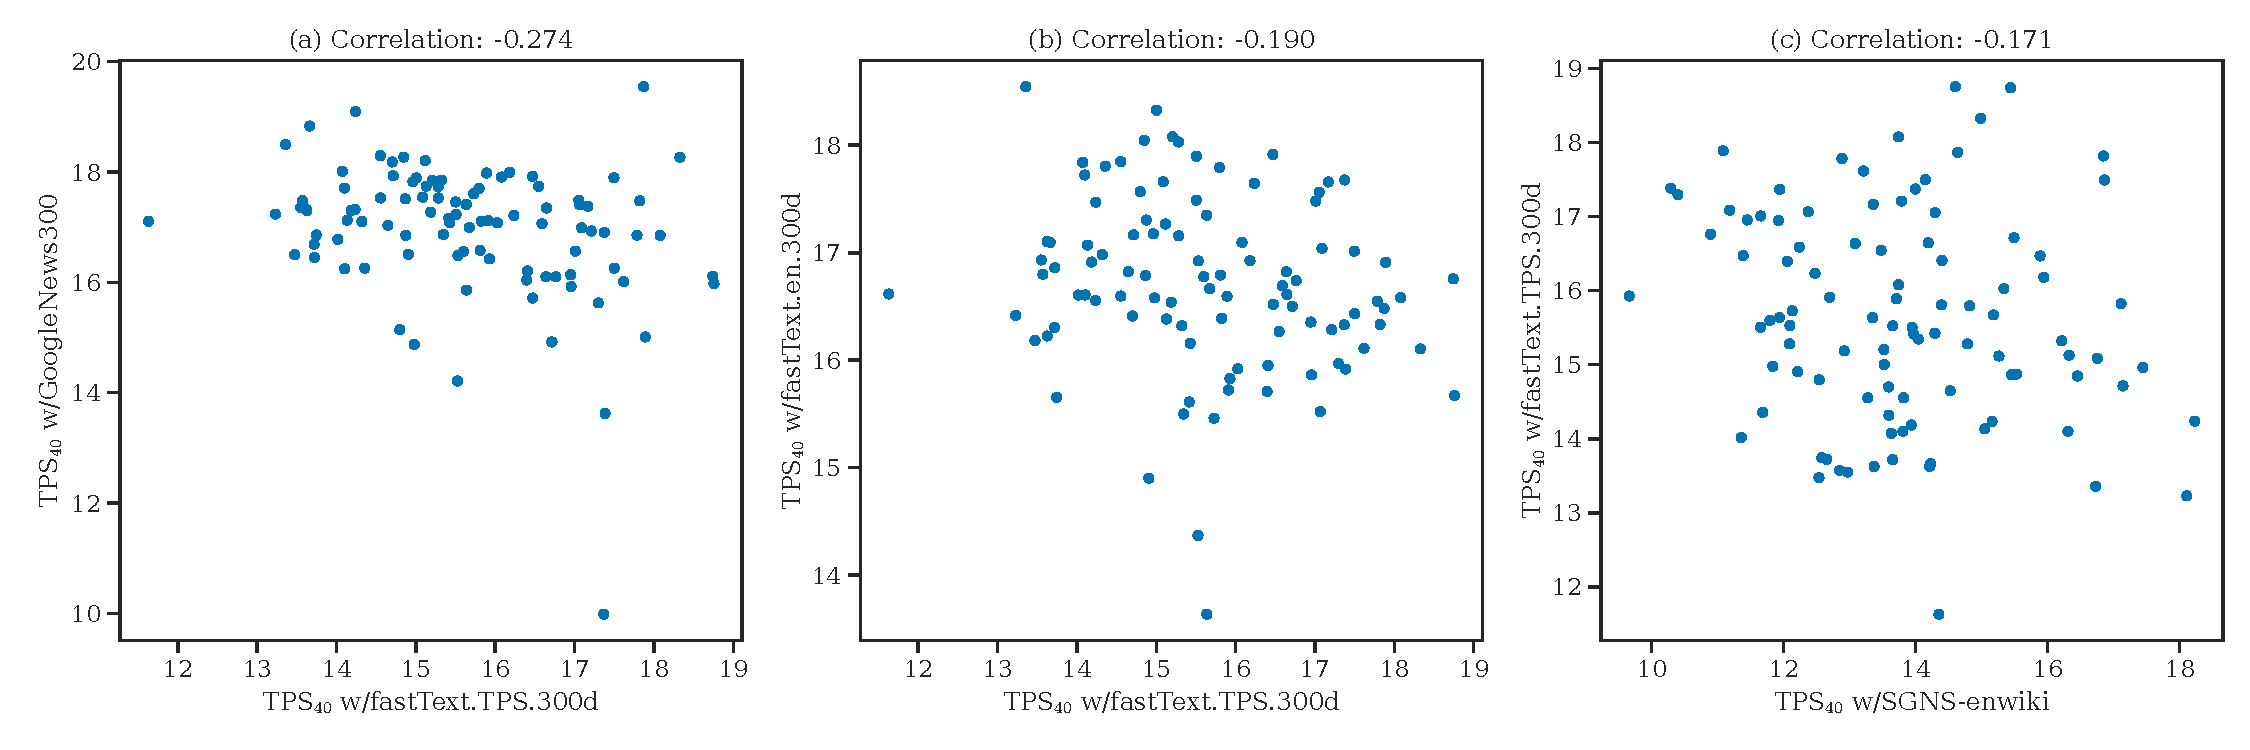
\includegraphics[width=\textwidth]{thesis/figures/tps-vs-gs-top-3-negative-correlation-word-embedding-models.pdf}
    \caption{$\text{TPS}_{40}(w)$ scores plotted against each other using the fastText.TPS.300d, GoogleNews300, fastText.en.300d and SGNS-enwiki models.}
    \label{fig:tps-vs-gs-top-3-negative-correlation-word-embedding-models}
\end{figure}

We have now looked at the effect of computing $\text{TPS}_n(w)$ at varying levels of $n$ using various word embeddings. We saw that, even by decreasing/increasing the vocabulary size of the word embedding models, the $\text{TPS}_n(w)$ score did not improve significantly. In all our experiments, except using the fastText.TPS.300d model, the correlation between $\text{TPS}_n(w)$ and the SemEval gold standard were always negative, while in the experiments of \cite{jakubowski2020topology}, they got a moderate, positive correlation. These results suggest that the topological polysemy scoring could be affected by the choice of word embedding model, i.e. choosing fastText over word2vec, and the fact that the model used in \cite{jakubowski2020topology} was trained on a data set that is strongly related to the 100 polysemous words from the SemEval task. In other words, it could seem that the measure of topological polysemy does not work well for a general word embedding model.

To deepen our understanding of how the $\text{TPS}_n(w)$ score is computed, we will perform an experiment by computing $\text{TPS}_n(w)$ of a custom data set. The custom data set consists of sampled data points of two spheres that share one intersection point. We denote this data set as \textit{2Spheres-$d$}, where $d$ represents the dimensionality of the spheres. In particular, we let $d \in \enclc{2, 3, 4, 5, 10, 20, 50, 300}$. To ensure that the dimensionality of the \textit{2Spheres-$d$} data set is similar to the dimensionality of word embeddings, we let the dimensionality of the space be equal to 300, i.e. \textit{2Spheres-$d$} $\in \R^{300}$. In other words, if $d$ was less than 300, we add zeros to the remaining dimensions to fill up to 300. For each sphere in \textit{2Spheres-$d$}, we generate 1000000 points on the sphere in $\R^d$. We sort the points by distance to the intersection point and split the points into 20 intervals, i.e. chunks of 100000 data points for each sphere. Next, we sample 1000 points from each interval, leading to 20000 points for each sphere. The motivation for sampling from intervals sorted by distance was to reduce the effect of the curse of dimensionality, namely that it becomes harder to measure the distance between points in high (e.g. 300) dimension. For the sake of simplicity, we let $n=50$ when computing the topological polysemy. We illustrate the result of computing $\text{TPS}_{50}$ of 2Spheres-$2$ and 2Spheres-$3$ in \cref{fig:two-spheres-2d-3d-tps-scores}. In \cref{fig:two-spheres-2d-3d-tps-scores}, we see that for both 2Spheres-$2$ and 2Spheres-$3$, the $\text{TPS}_{50}$ is at its highest (yellow color) around the intersection point between the two spheres (see \cref{fig:two-spheres-2d-3d-tps-scores} (b) and (d)). In addition to this, at the intersection point between the two spheres, the $\text{TPS}_{50}$ score is low. These two observations suggest that for low values of $d$, the $\text{TPS}_{50}$ score fails to identify the singular point and instead manages to identify the area around it. We will now look at how the $\text{TPS}_{50}$ score behaves for $d \in \enclc{4, 5, 10, 20, 50, 300}$.
\begin{figure}[H]
    \centering
    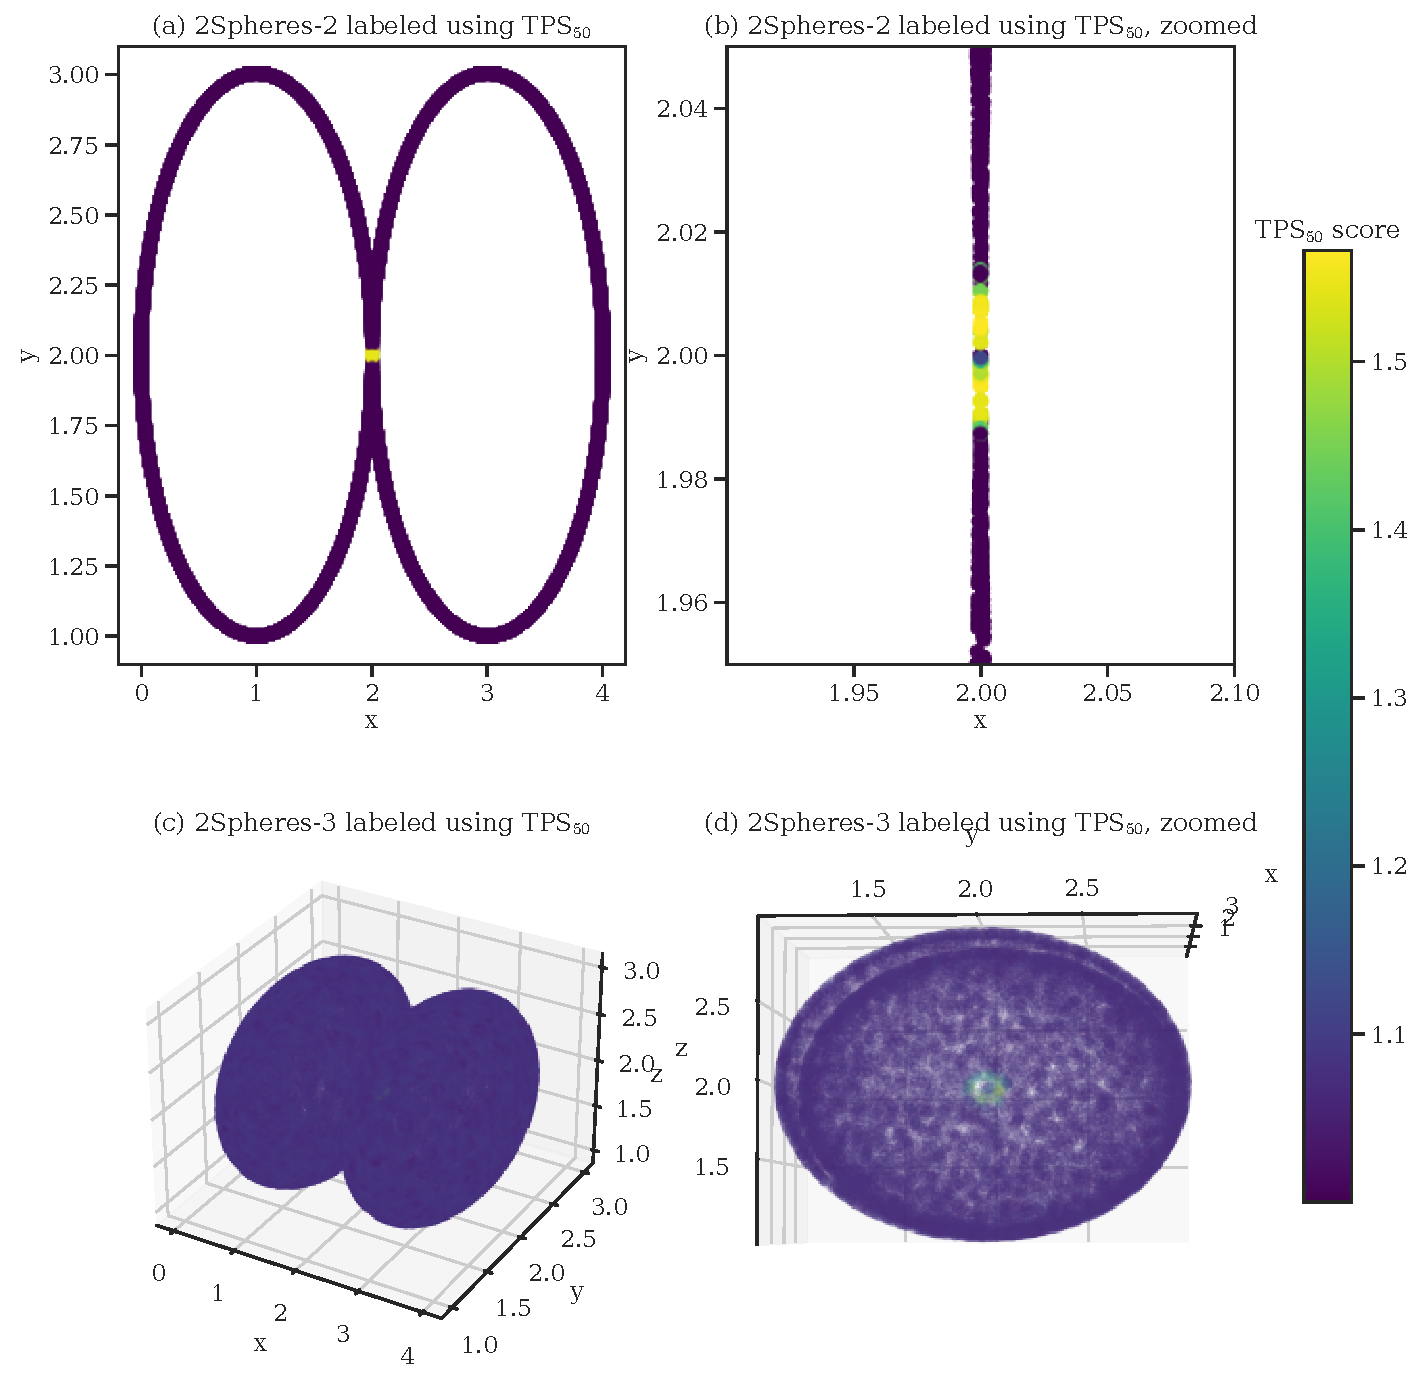
\includegraphics[width=\textwidth]{thesis/figures/two-spheres-2d-3d-tps-scores.pdf}
    \caption{Plots of the 2Spheres-$2$ and 2Spheres-$3$ data sets, with $\text{TPS}_{50}$ as labels. The intersection point between the spheres is at $(2, 2)$ in 2 dimensions and at $(2, 2, 2)$ in 3 dimensions.}
    \label{fig:two-spheres-2d-3d-tps-scores}
\end{figure}

We visualize the result of computing $\text{TPS}_{50}$ for 2Spheres-$d$ for $d \in \enclc{4, 5, 10, 20, 50, 300}$ in \cref{fig:two-spheres-distance-to-int-point-vs-tps-scores}, by plotting the distance to the intersection point between the spheres against the $\text{TPS}_{50}$ scores. In \cref{fig:two-spheres-distance-to-int-point-vs-tps-scores}, we see that as the dimension of the spheres increases, the "peak" of $\text{TPS}_{50}$ scores close to the intersection point diminishes. The diminishing effect comes due to the curse of dimensionality (\cref{fig:curse-of-dimensionality}), namely that in high dimensional space, all distances become very similar, as seen in \cref{fig:two-spheres-distance-to-int-point-vs-tps-scores} (f). In other words, for high dimensional spheres, it becomes difficult to identify the intersection point between the spheres, using the $\text{TPS}_{50}$ scores, as the distances become similar, and $\text{TPS}_{50}$ is unable to identify areas around the intersection point, which we saw happening in lower dimensions (\cref{fig:two-spheres-2d-3d-tps-scores}). We note, however, however, that for high values of $d$, the intersection point has a $\text{TPS}_{50}$ score which generally is higher than all other values of $\text{TPS}_{50}$. Finally, we argue that these results shown in \cref{fig:two-spheres-distance-to-int-point-vs-tps-scores} indicates that the topological measure of polysemy may suffer when applied to high-dimensional (e.g. 300) data.
\begin{figure}[H]
    \centering
    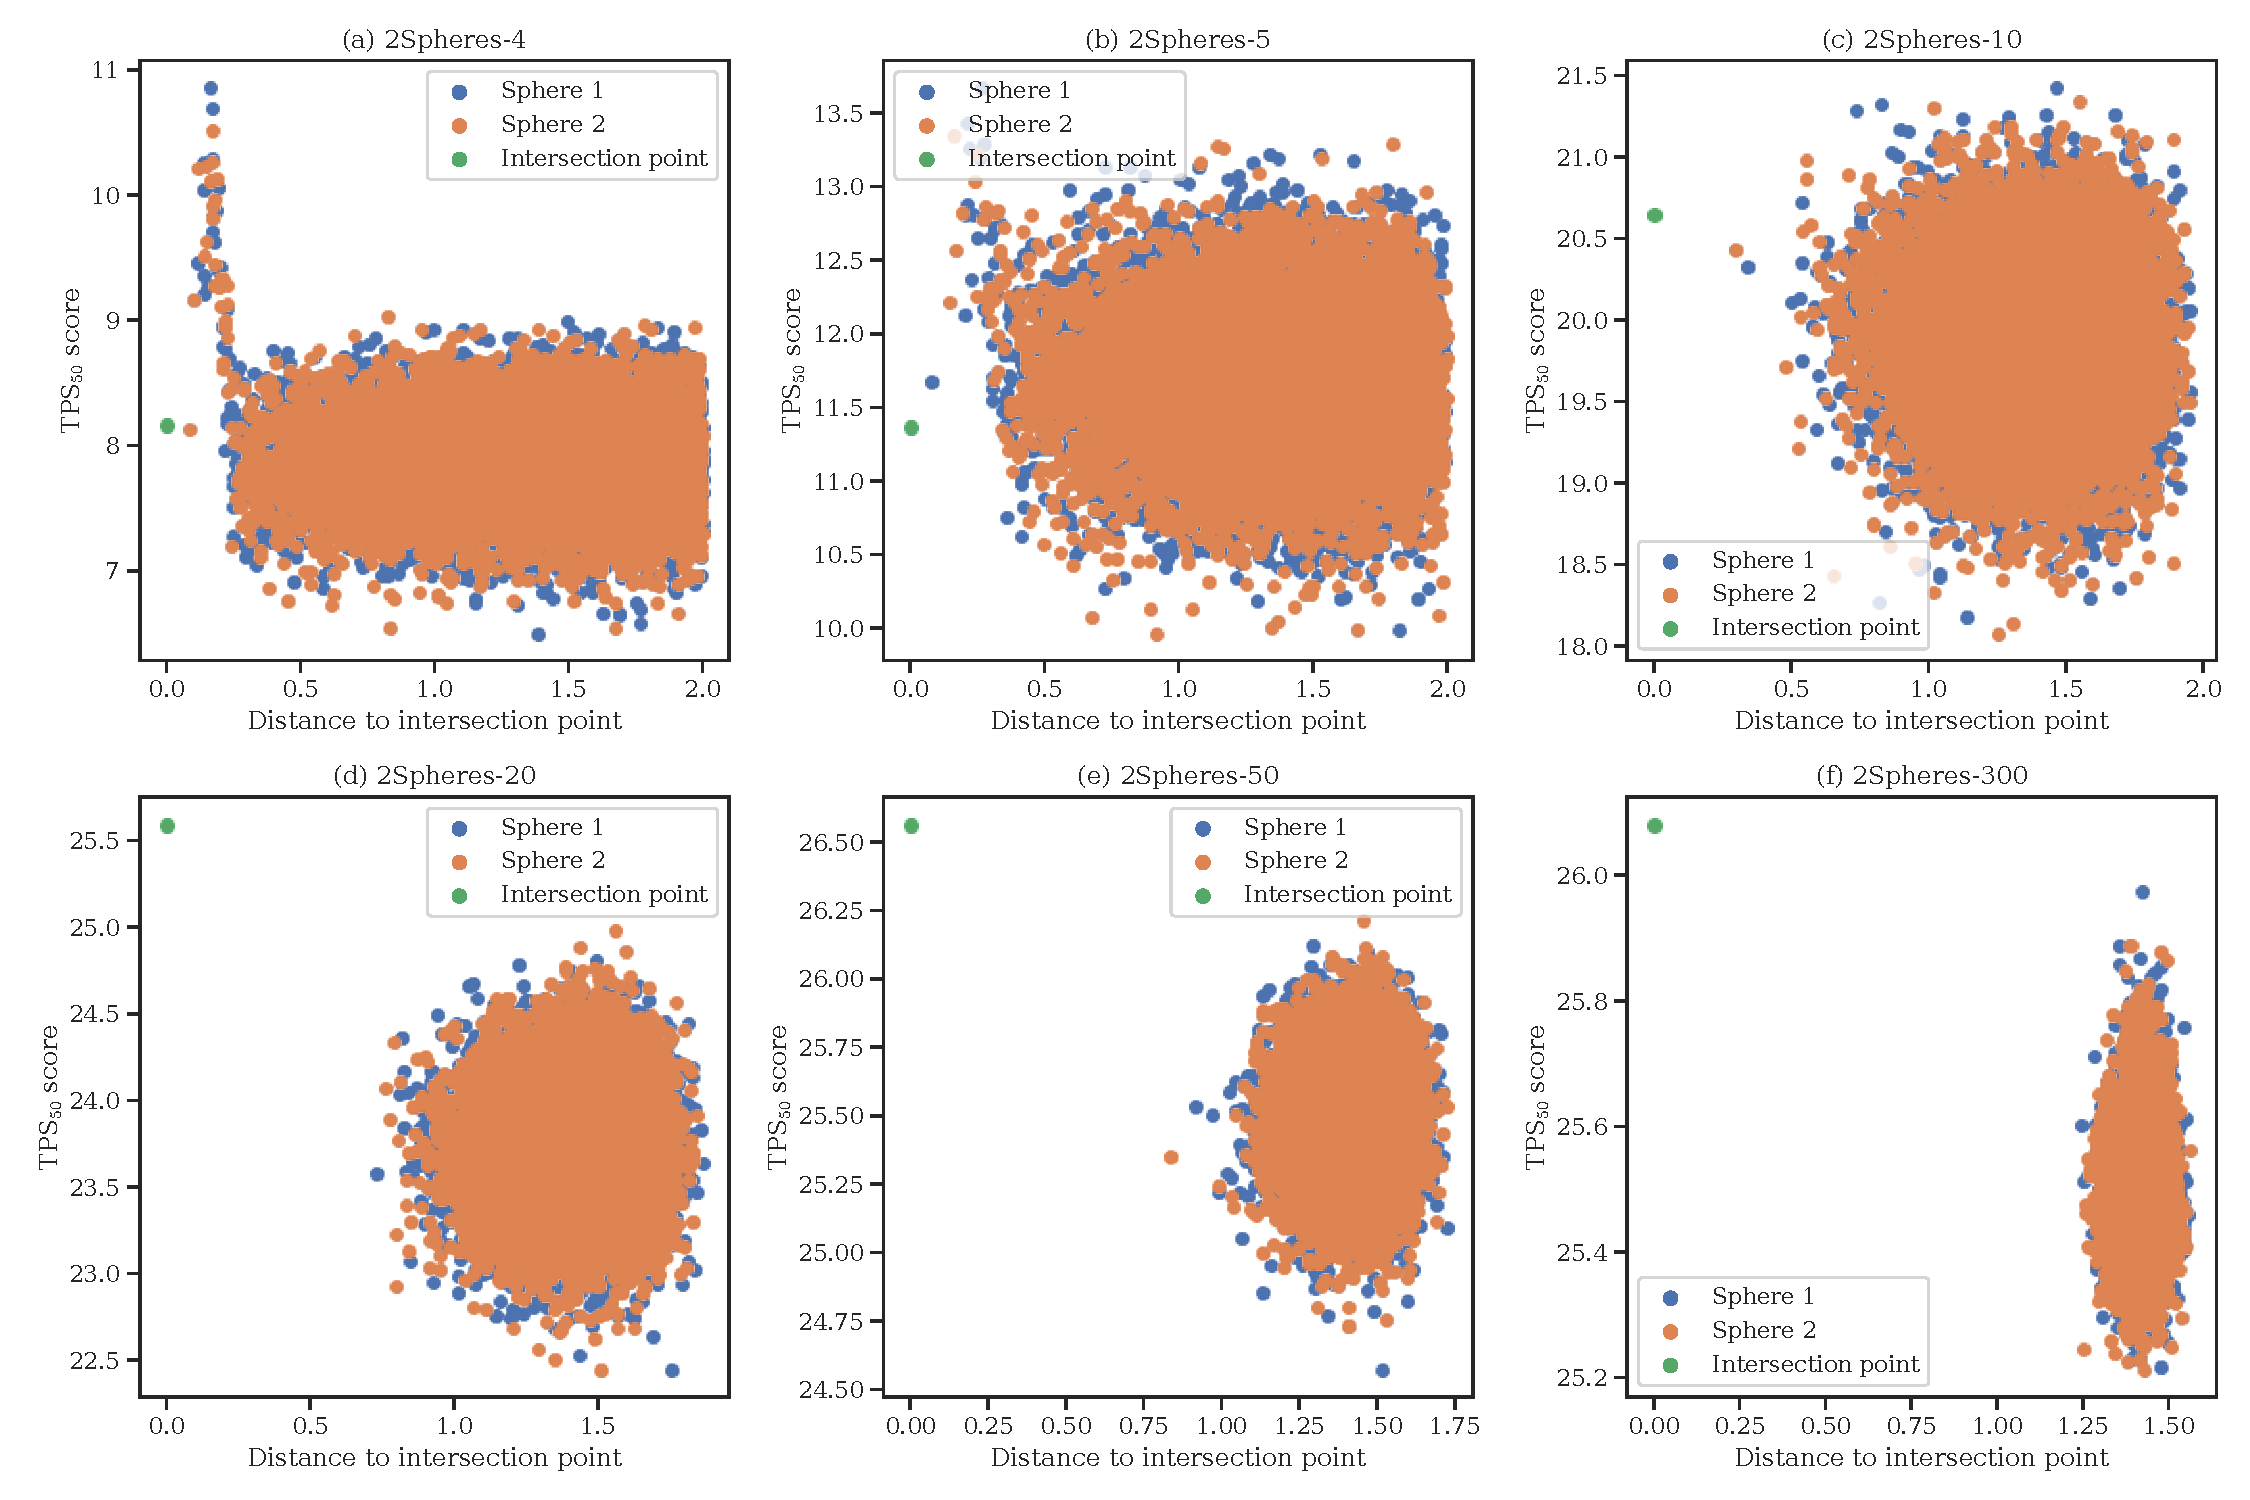
\includegraphics[width=\textwidth]{thesis/figures/two-spheres-distance-to-int-point-vs-tps-scores.pdf}
    \caption{Distance to the intersection point between spheres plotted against $\text{TPS}_{50}$ scores for 2Spheres-$d$, $d \in \enclc{4, 5, 10, 20, 50, 300}$.}
    \label{fig:two-spheres-distance-to-int-point-vs-tps-scores}
\end{figure}

Following, we repeated the experiment where we computed the topological polysemy of two spheres. In particular, we used a noisy version of the 2Spheres-$d$ data set, which we denoted as the \textit{2SpheresNoisy-$d$} data set. The motivation for adding some noise to the spheres data set was to emulate some real-world effect, namely that data sets are usually not uniformly distributed in practice. In particular, the 2SpheresNoisy-$d$ data set was created by perturbing the 2Spheres-$d$ data set by adding Gaussian noise at every data point. In particular, we used Gaussians with zero mean and a variance of 0.1. We first computed the $\text{TPS}_{50}$ score of the 2SpheresNoisy-$2$ and 2SpheresNoisy-$3$ data sets. We show the results in \cref{fig:two-spheres-noisy-2d-3d-tps-scores}, where we see that in the 2-dimensional case, the $\text{TPS}_{50}$ scores are high (i.e. yellow colour) and we are unable to identify the intersection point between the spheres. Moreover, in \cref{fig:two-spheres-noisy-2d-3d-tps-scores} (c) and (d) we see that the $\text{TPS}_{50}$ scores are mediocre at best, and we are unable to identify the intersection point between the spheres. The results in \cref{fig:two-spheres-noisy-2d-3d-tps-scores} tells us that if we perturb the data set by adding noise, it becomes harder to identify singular points in lower dimensions ($d \in \enclc{2, 3}$), when compared to the $\text{TPS}_{50}$ results using 2Spheres-$d$, which we show in \cref{fig:two-spheres-2d-3d-tps-scores}.
\begin{figure}[H]
    \centering
    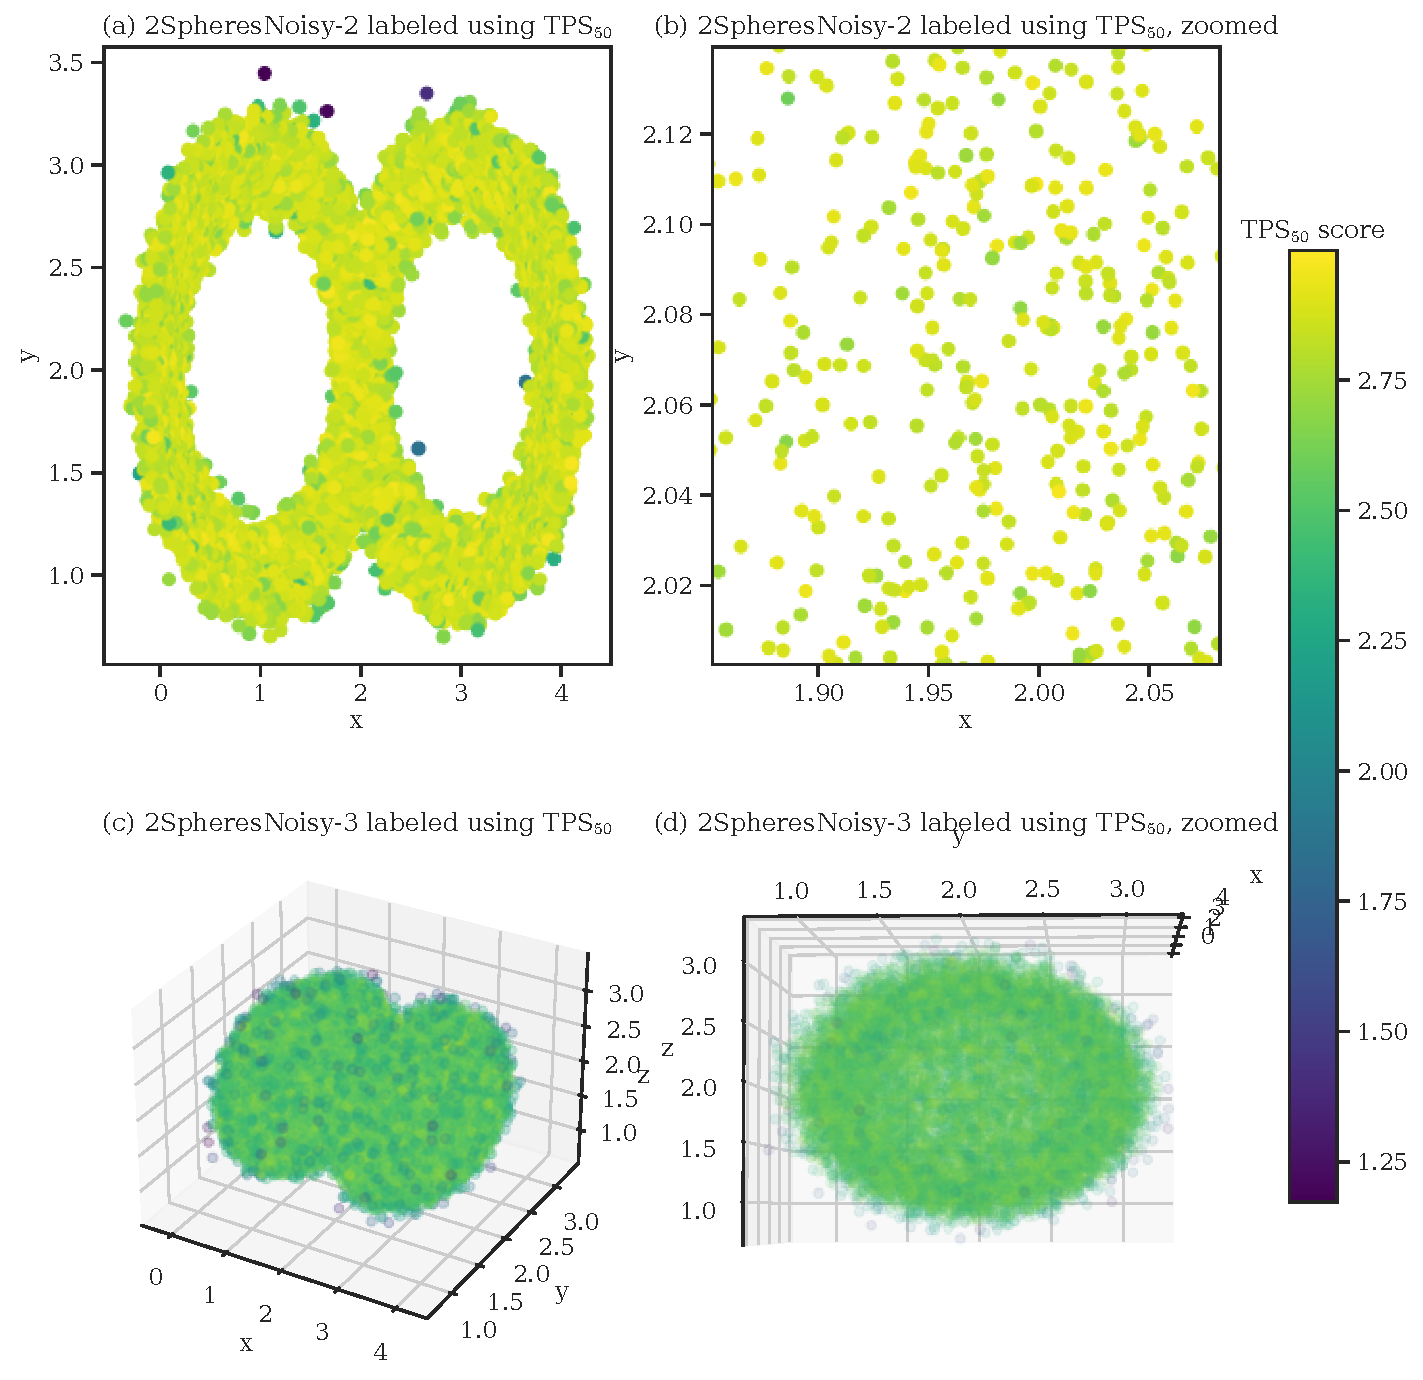
\includegraphics[width=\textwidth]{thesis/figures/two-spheres-noisy-2d-3d-tps-scores.pdf}
    \caption{Plots of the 2SpheresNoisy-$2$ and 2SpheresNoisy-$3$ data sets, with $\text{TPS}_{50}$ as labels. The intersection point between the spheres is at $(2, 2)$ in 2 dimensions and at $(2, 2, 2)$ in 3 dimensions.}
    \label{fig:two-spheres-noisy-2d-3d-tps-scores}
\end{figure}

Finally, we visualize the result of computing $\text{TPS}_{50}$ for 2SpheresNoisy-$d$ for $d \in \enclc{4, 5, 10, 20, 50, 300}$ in \cref{fig:two-spheres-noisy-distance-to-int-point-vs-tps-scores}, by plotting the distance to the intersection point between the spheres against the $\text{TPS}_{50}$ scores. In \cref{fig:two-spheres-noisy-distance-to-int-point-vs-tps-scores}, we see a similar situation appearing to the results using 2Spheres-$d$ in \cref{fig:two-spheres-distance-to-int-point-vs-tps-scores}. In particular, we observe that as we increase the dimensionality of the spheres towards 300, the distances to the intersection point becomes more or less the same, and it is difficult to differentiate between the intersection point and regular points on the two spheres. We note, however, that in \cref{fig:two-spheres-noisy-distance-to-int-point-vs-tps-scores} (f) we see that the $\text{TPS}_{50}$ score is significantly larger than the rest of the $\text{TPS}_{50}$ scores and it could be possible to identify the intersection point using its $\text{TPS}_{50}$ score. Although this result might seem significant in \cref{fig:two-spheres-noisy-distance-to-int-point-vs-tps-scores} (f), the 2SpheresNoisy-$d$ is still rather simple when compared to real-world word embeddings, even when we added the noise. Additionally, the significance we show in \cref{fig:two-spheres-noisy-distance-to-int-point-vs-tps-scores} (f) can be due to a random effect of the 2SpheresNoisy-300 data set.
\begin{figure}[H]
    \centering
    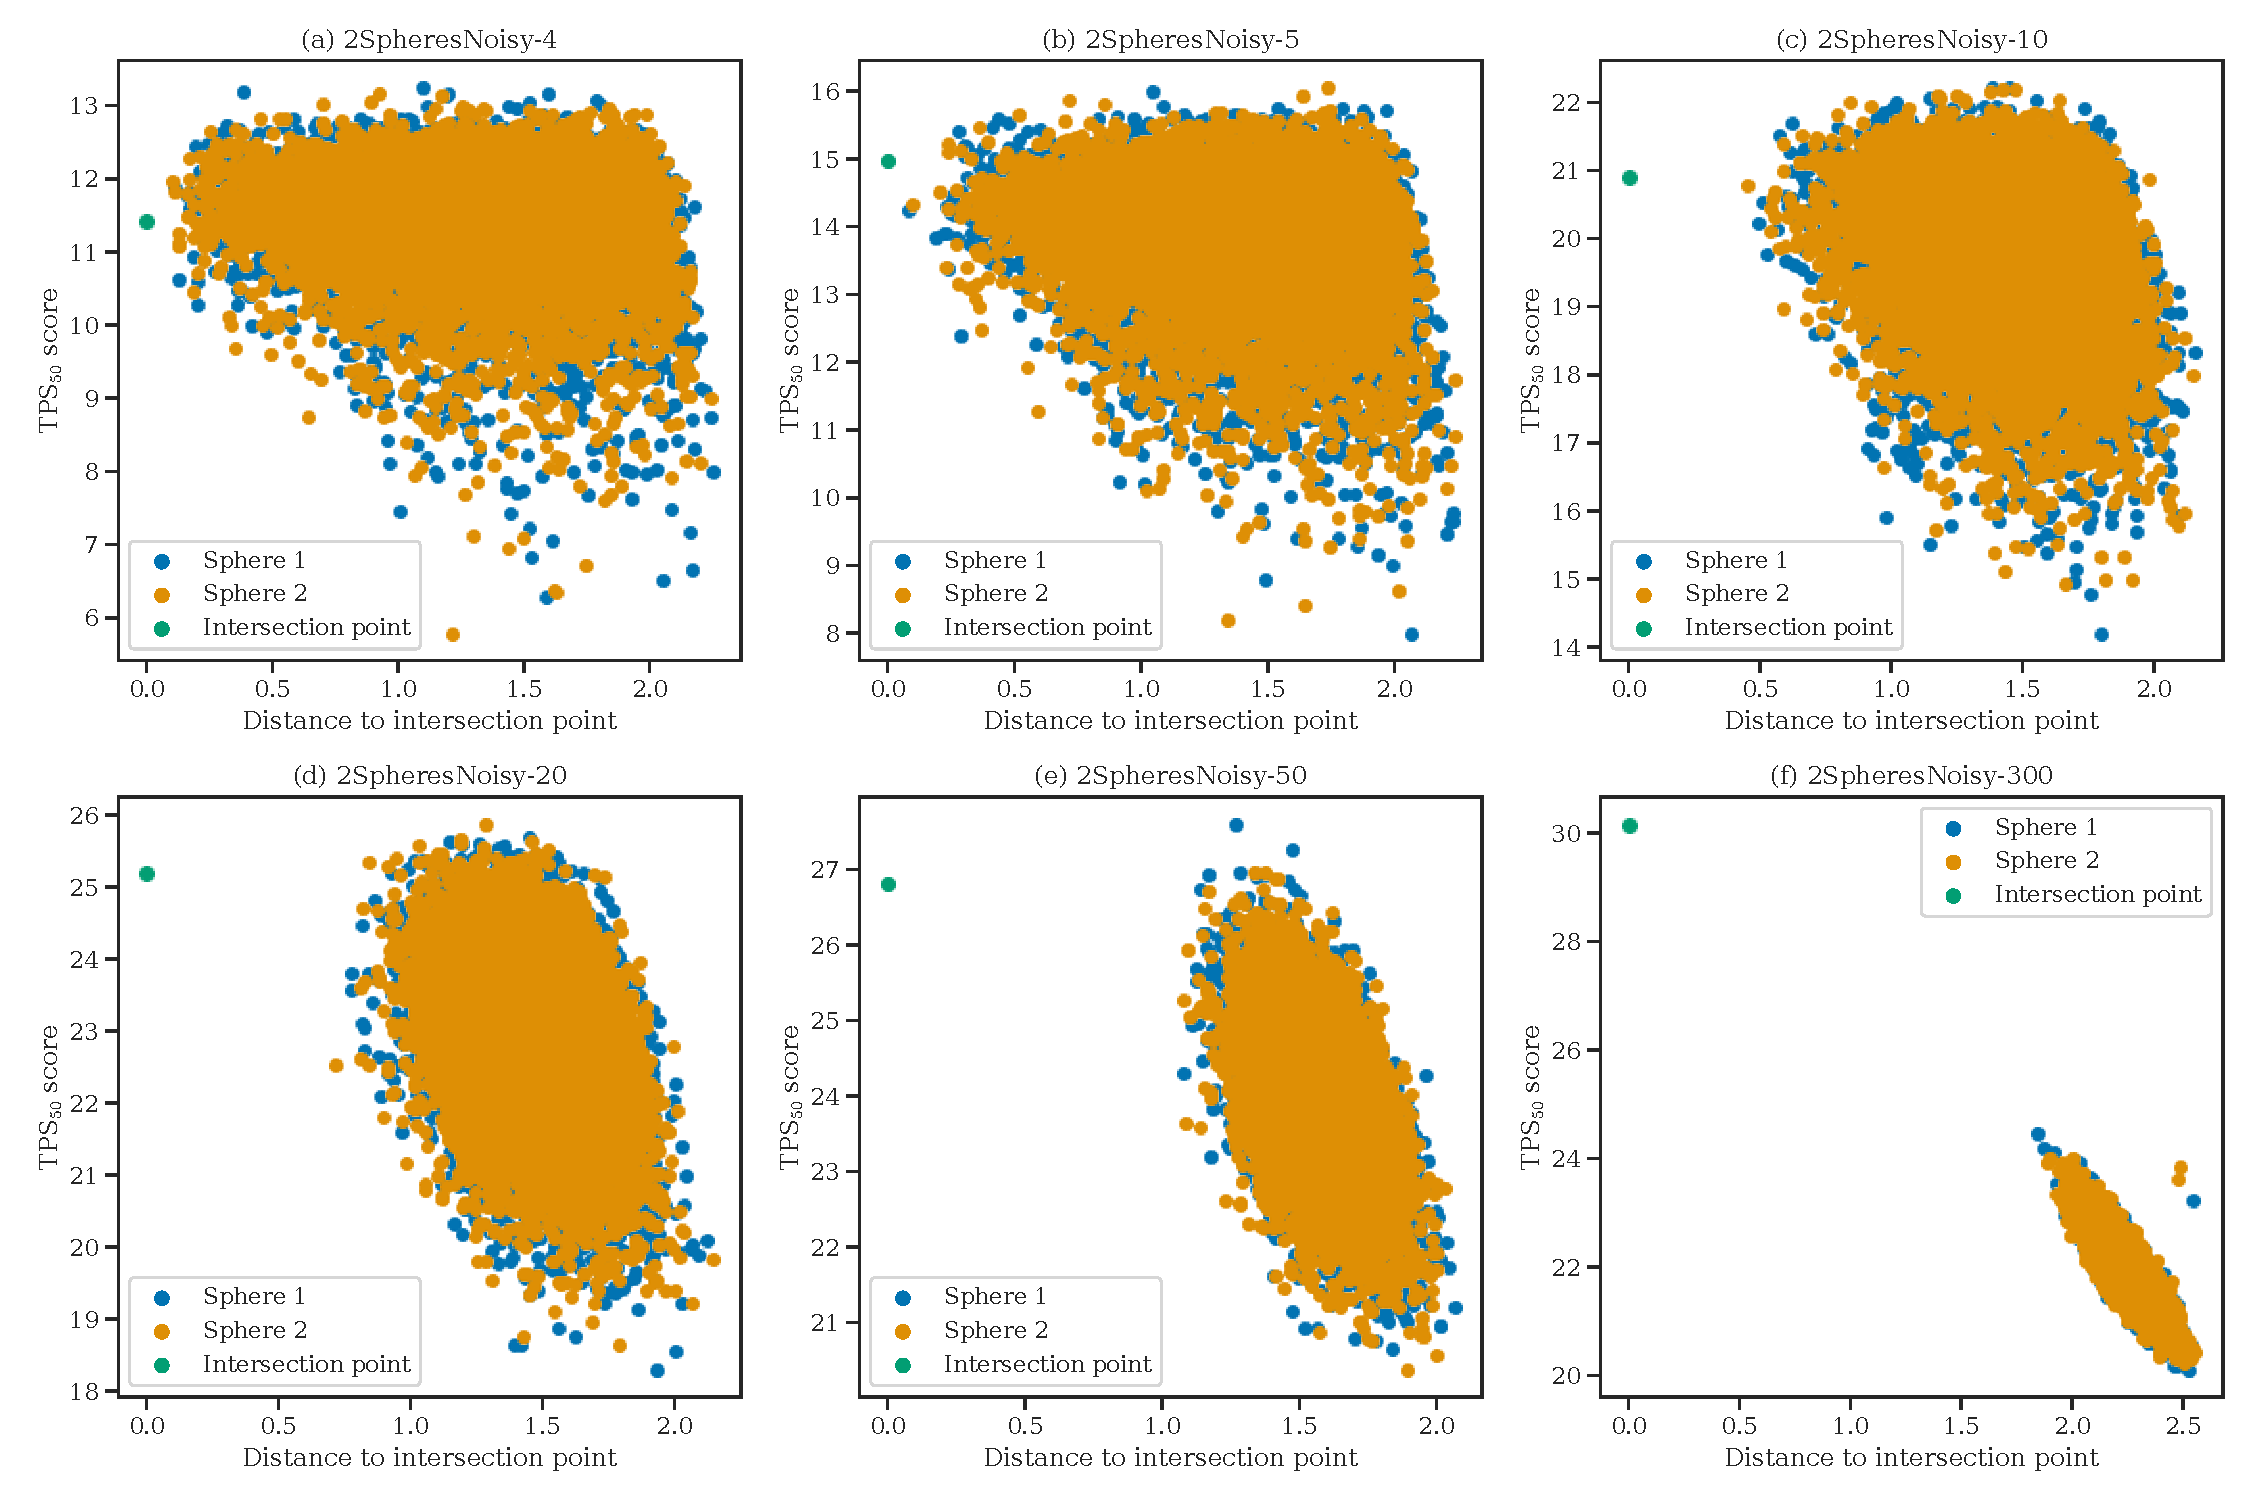
\includegraphics[width=\textwidth]{thesis/figures/two-spheres-noisy-distance-to-int-point-vs-tps-scores.pdf}
    \caption{Distance to the intersection point between spheres plotted against $\text{TPS}_{50}$ scores for 2SpheresNoisy-$d$, $d \in \enclc{4, 5, 10, 20, 50, 300}$.}
    \label{fig:two-spheres-noisy-distance-to-int-point-vs-tps-scores}
\end{figure}

Furthermore, we will use the measure of topological polysemy when we create supervised models for the prediction of polysemous words in \cref{sec:analysis-of-embeddings-supervised-polysemy-prediction}. Next, we will look at Geometric Anomaly Detection, and in particular, how it performs when applied to word embeddings.

\subsection{Geometric Anomaly Detection}
\label{sec:analysis-of-embeddings-geometric-anomaly-detection}
In this subsection, we will apply the Geometric Anomaly Detection (GAD) (\cref{sec:geometric-anomaly-detection}) algorithm to the word embeddings from the SGNS-enwiki model. In particular, we will show the relationship between how GAD categorizes word embeddings into groups and whether words are polysemous. We implemented GAD as explained in \cref{sec:geometric-anomaly-detection}, using similar packages to the ones we used to implement topological polysemy in \cref{sec:analysis-of-embeddings-topological-polysemy}. In particular, we used the ScaNN \cite{scann2020} approximate nearest neighbour algorithm, to speed up the nearest-neighbour computation, and \path{ripser} \cite{ctralie2018ripser} Python package, to compute Vietoris–Rips complexes. We also included an option to use the Ripser++ \cite{zhang2020ripserplusplus} Python package instead of \path{ripser}, which is a GPU accelerated version of \path{ripser}. However, we quickly found that the GPU overhead was too big and it was faster just to use the regular \path{ripser} Python package.

Before applying GAD to word embeddings, we will motivate the use of GAD by visualizing GAD applied to the 3-dimensional \textit{Henneberg surface} data set, as used in the experiments of \cite{stolz2020geometric}. To compute the GAD of the Henneberg surface data set, we used the same hyperparameters as in \cite{stolz2020geometric}, that is, we let the inner annulus radius equal 1.5, outer annulus radius equal 2 and the manifold dimension $k$ equal 2. We visualize the result in \cref{fig:gad-henneberg-3d}, where we see how GAD groups data points to the manifold, boundary and singular groups. In the 3-dimensional Henneberg surface data set, there are four 2-dimensional surfaces that intersect, as we see in \cref{fig:gad-henneberg-3d} (b), which the GAD algorithm managed to correctly identify as singular points. In addition to the singular points, the boundary points are also nicely shown in both \cref{fig:gad-henneberg-3d} (a) and (b).
\begin{figure}[H]
    \centering
    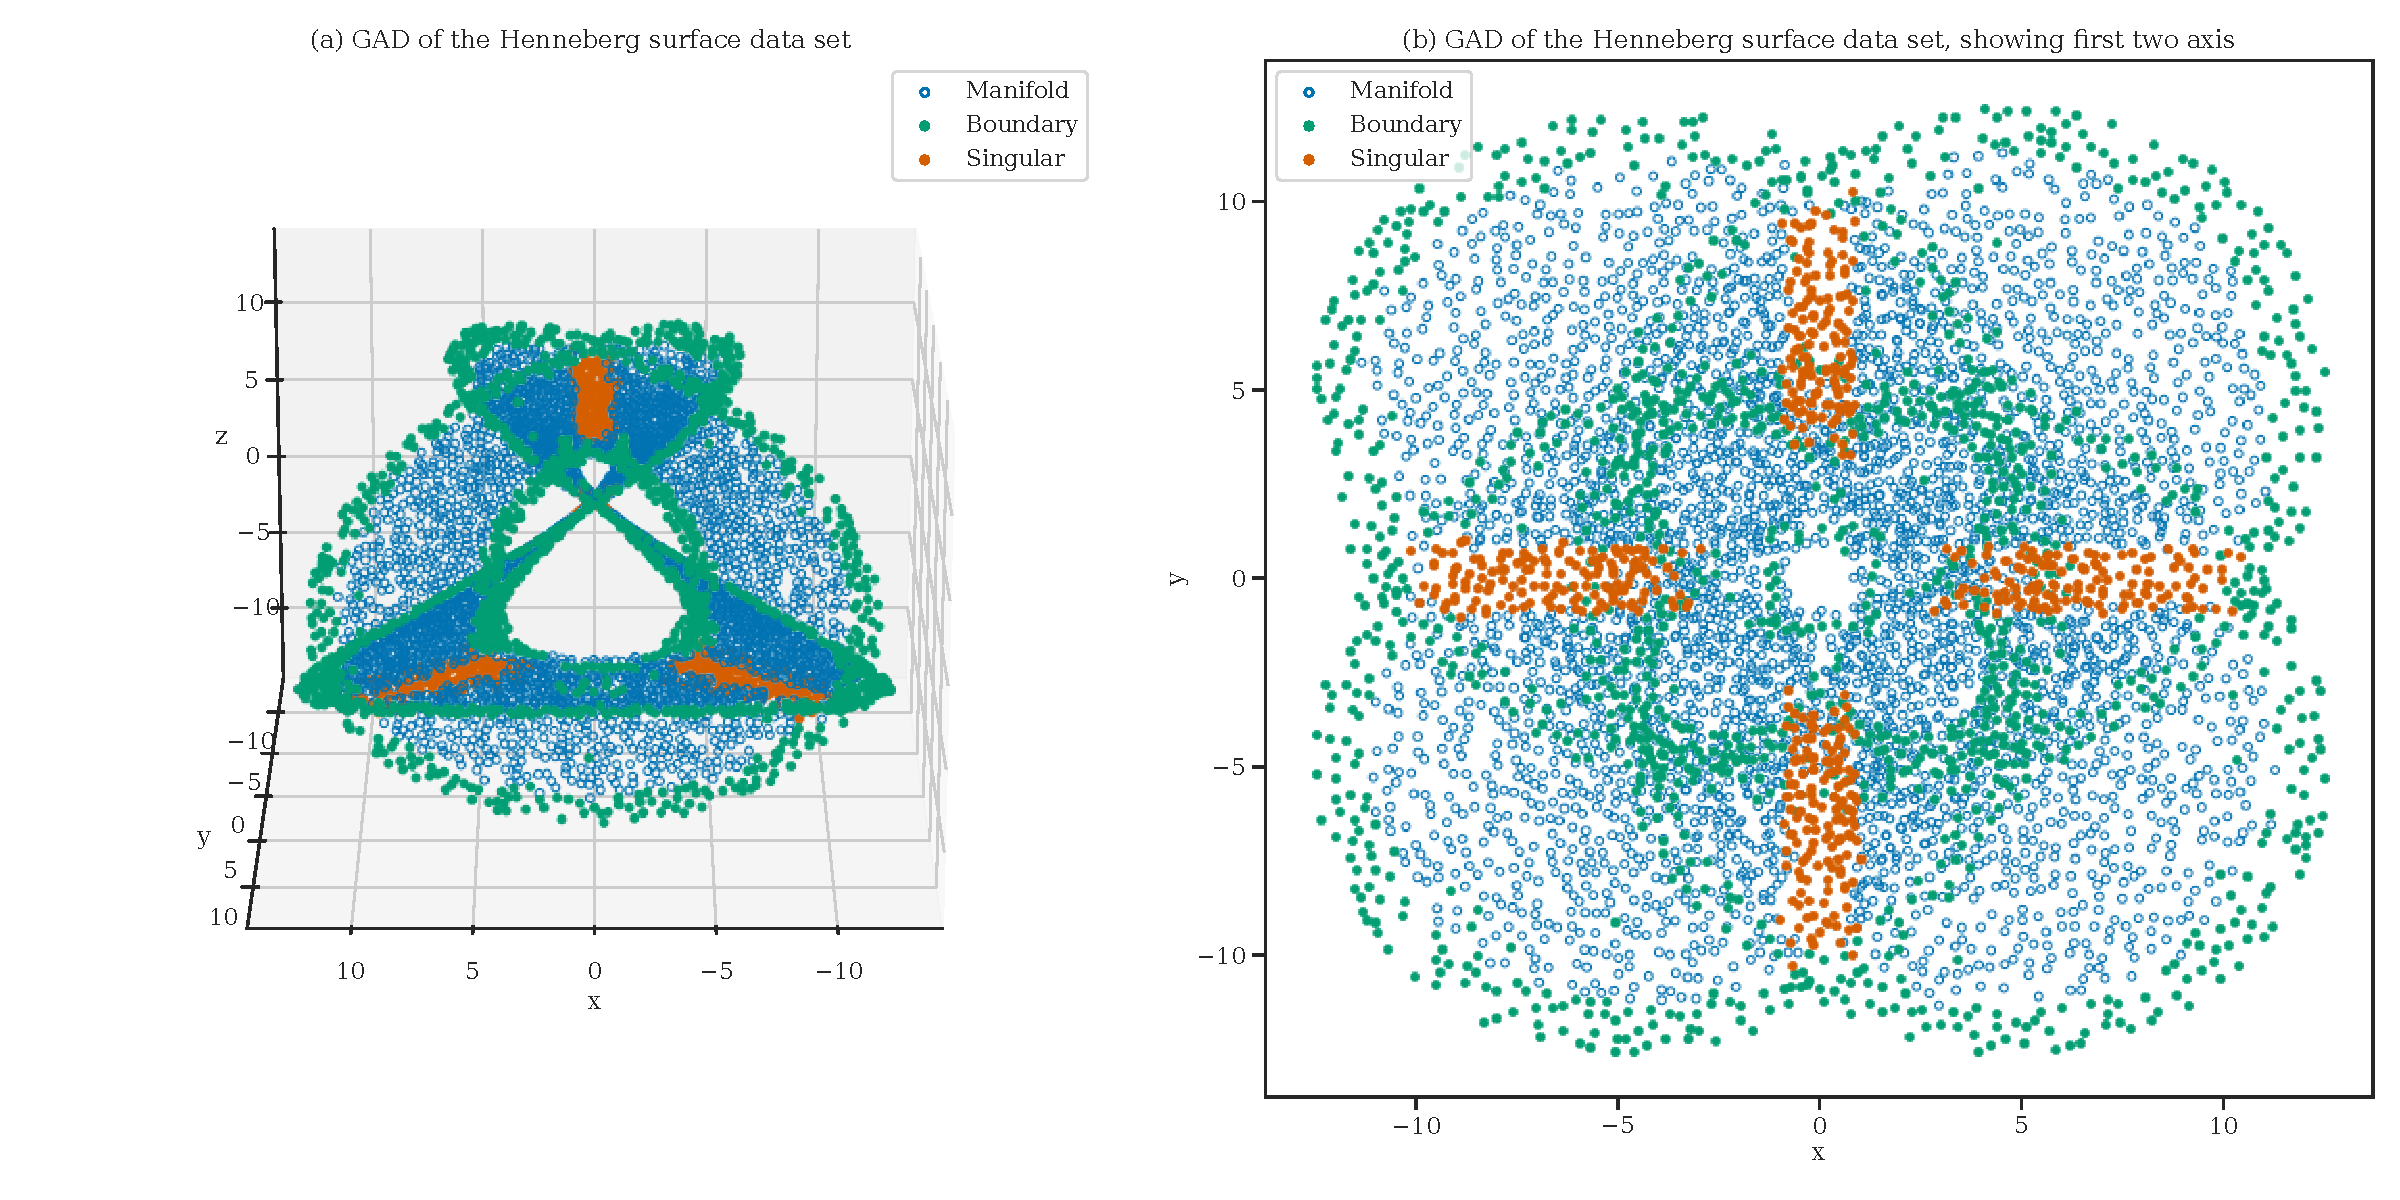
\includegraphics[width=\textwidth]{thesis/figures/gad-henneberg-3d.pdf}
    \caption{2D and 3D projections of the Henneberg surface data set, labelled with the data point groups from the GAD algorithm. This figure is inspired by \cite[Figure 3]{stolz2020geometric}.}
    \label{fig:gad-henneberg-3d}
\end{figure}

Following, we visualize the Henneberg surface data set with the $\text{TPS}_{50}$ score computed for each point. In \cref{fig:gad-henneberg-3d-tps-50}, we see that the $\text{TPS}_{50}$ scores fails to identify the singular data points if the Henneberg surface data set,which we expected to have relatively high $\text{TPS}_{50}$ scores. In particular, the $\text{TPS}_{50}$ scores are relatively high for points on the manifold, and lower for the boundary and singular points.
\begin{figure}[H]
    \centering
    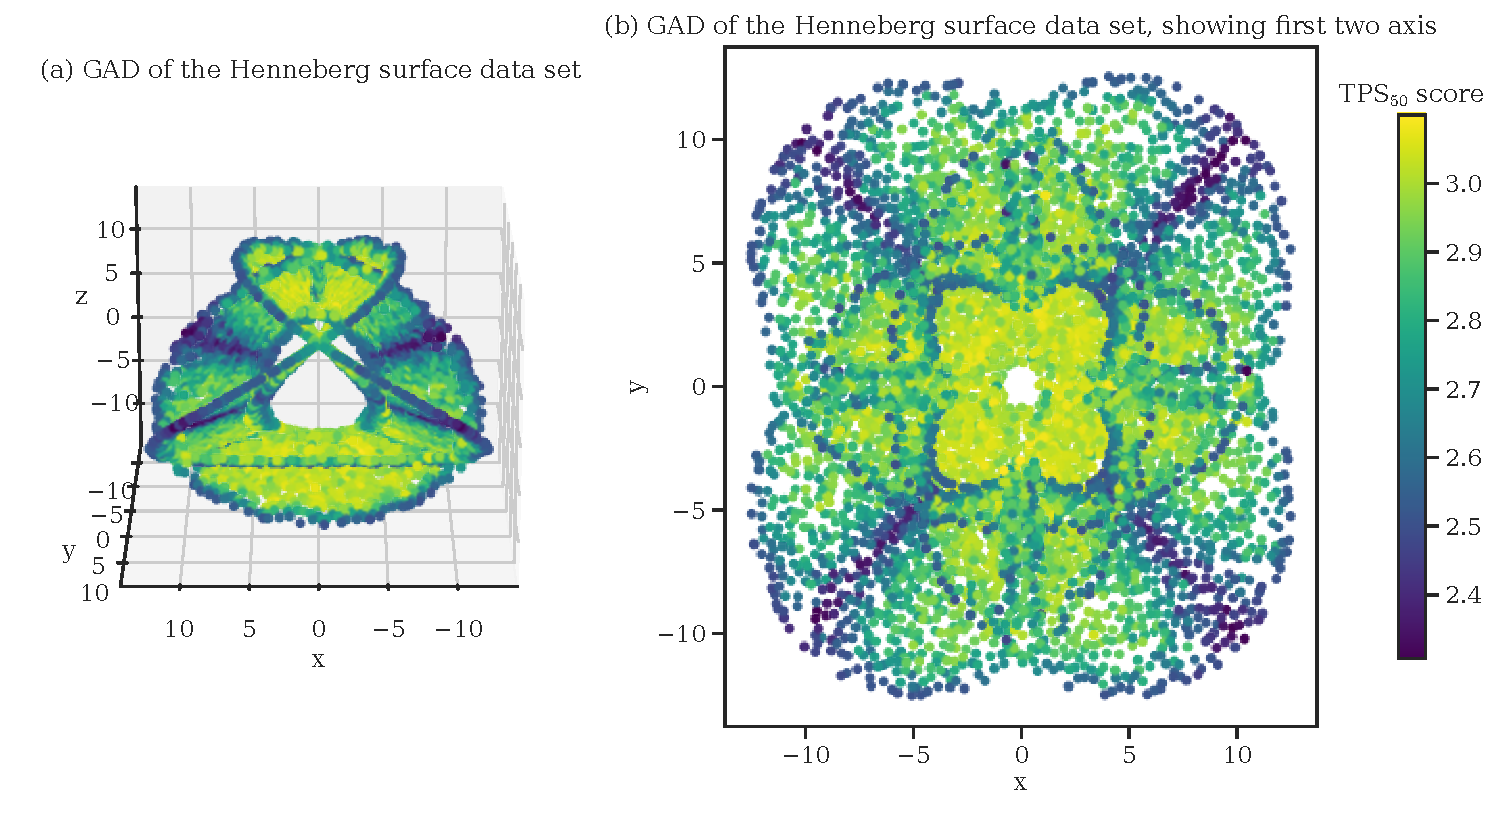
\includegraphics[width=\textwidth]{thesis/figures/gad-henneberg-3d-tps-50.pdf}
    \caption{2D and 3D projections of the Henneberg surface data set, labelled with the $\text{TPS}_{50}$ score for each point.}
    \label{fig:gad-henneberg-3d-tps-50}
\end{figure}

We will now apply GAD to the word embeddings from the SGNS-enwiki model. In particular, we will apply GAD to the words that have a WordNet entry, similar to how we performed the topological polysemy experiments on SGNS-enwiki word embeddings in \cref{sec:analysis-of-embeddings-topological-polysemy}. Furthermore, the standard GAD algorithm uses annulus radii parameters to do its computation, and because it is unknown which radii parameters to use for a general data set, we will instead default to a $k$-nearest neighbour approach when computing GAD of the WordNet SGNS-enwiki word embeddings. Using the $k$-nearest neighbour approach, we let the inner annulus radius equal the distance to the $s$ nearest neighbour of each word, and similarly for the outer annulus radius, which we set equal to the distance to the $t$ nearest neighbour of each word. To apply GAD to the WordNet SGNS-enwiki word embeddings, we used the parameters $s=25$ and $t=500$. We show the number of words in each GAD group in \cref{table:number-of-words-gad-polysemous-sgns-enwiki-wordnet}. In \cref{table:number-of-words-gad-polysemous-sgns-enwiki-wordnet}, we see that the number of polysemous WordNet words that fall into the singular group is particularly low; only 344 of 48880. In addition to this, we see that the number of words being categorized as "boundary" words is high. These two observations suggest that our inner and outer annulus radius, as well as the manifold dimension $k$, were not set correctly for the data set we are applying GAD to. Keep in mind that the intrinsic dimensionalities of word embeddings are most likely higher than $k=2$, but due to the computational cost of setting $k > 2$ (creation of the Vietoris–Rips complex), we will not set $k$ greater than 2 in this thesis.
\begin{table}[H]
    \centering
    \begin{tabular}{@{}lcccl@{}}
    \toprule
    \multicolumn{1}{c}{}       & \multicolumn{3}{c}{GAD group}  & \multicolumn{1}{l}{} \\ \cmidrule(lr){2-4}
    \multicolumn{1}{c}{}       & Manifold & Boundary & Singular & \textit{Sum}                  \\ \midrule
    \trcolor Number of monosemous words            & 4 640     & 86 731    & 4 161     & 95 532                \\
    Number of polysemous words & 634      & 47 902    & 344      & 48 880                \\ \midrule
    \trcolor \textit{Sum}                        & 5 274     & 134 633   & 4 505     & 144 412 \\ \bottomrule
    \end{tabular}
    \caption{Number of monosemous and polysemous words in each GAD group, when applied to the WordNet SGNS-enwiki word embeddings.}
    \label{table:number-of-words-gad-polysemous-sgns-enwiki-wordnet}
\end{table}

Finally, we visualize the result using a 2-dimensional UMAP embedding of the 10000 most common words of the WordNet SGNS-enwiki word embeddings in \cref{fig:gad-umap-2d-10k-most-common-wordnet-enwiki-words}, which we labelled using the GAD groups. In \cref{fig:gad-umap-2d-10k-most-common-wordnet-enwiki-words}, we see that only a single word is categorized to be singular (the word "branch"), some words are categorized to be on the manifold, and the rest are categorized to be on the boundary. These results indicate that the hyperparameters we used to compute GAD are not suitable for the data set at hand. We also observe that \cref{fig:gad-umap-2d-10k-most-common-wordnet-enwiki-words} differs a whole lot from GAD applied to the Henneberg surface data set (\cref{fig:gad-henneberg-3d}), which indicates bad hyperparameterization.
\begin{figure}[H]
    \centering
    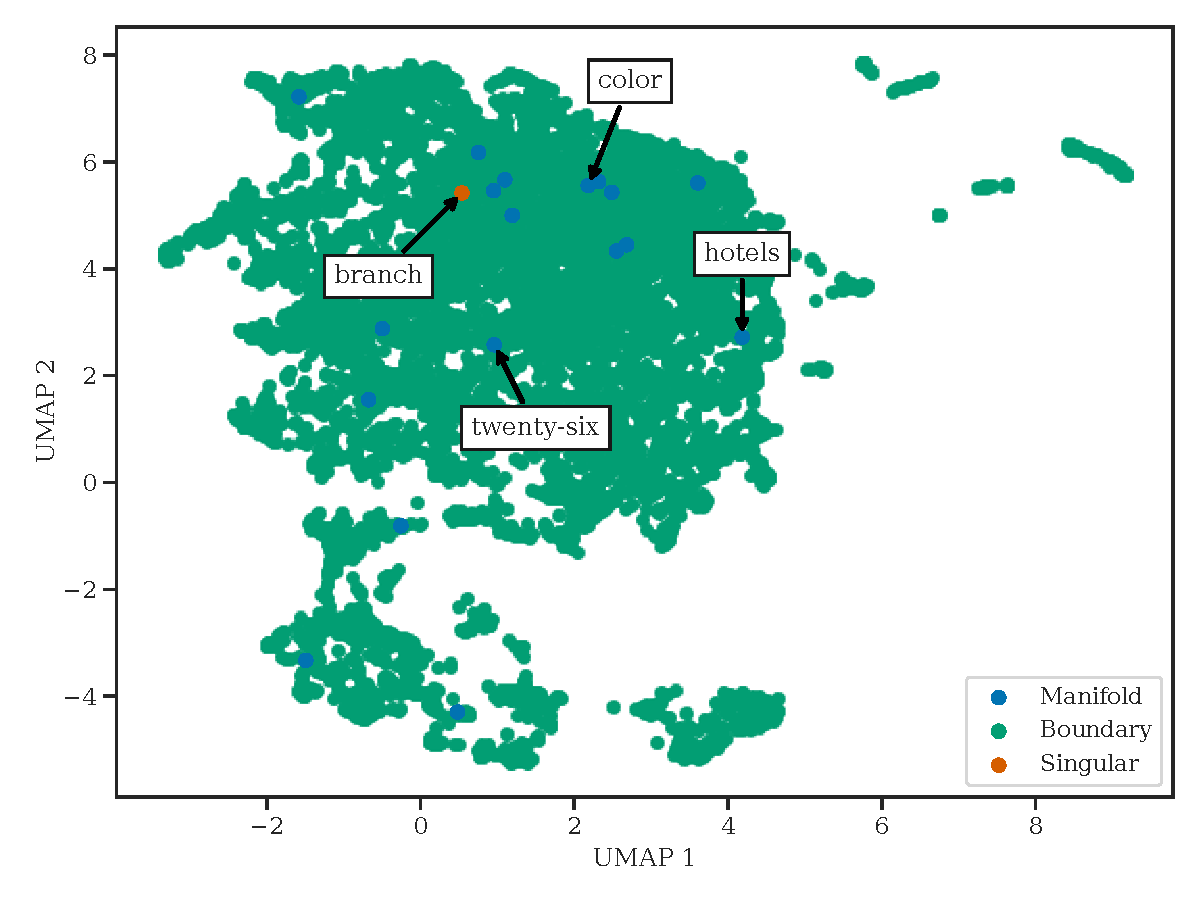
\includegraphics[width=0.8\textwidth]{thesis/figures/gad-umap-2d-10k-most-common-wordnet-enwiki-words.pdf}
    \caption{2-dimensional UMAP embedding of the 10000 most common words of the WordNet SGNS-enwiki word embeddings. The words are labelled using their GAD group.}
    \label{fig:gad-umap-2d-10k-most-common-wordnet-enwiki-words}
\end{figure}

Furthermore, we will investigate the effect of using different sets of hyperparameters when applying GAD to word embeddings in \cref{sec:analysis-of-embeddings-supervised-polysemy-prediction}, where we create supervised models for predicting whether or not a word is polysemous. Next, we will investigate algorithms for estimating the intrinsic dimensionality of word embeddings, and how it correlates with the actual number of word meanings.

\subsection{Intrinsic dimension estimation}
\label{sec:analysis-of-embeddings-intrinsic-dimension-estimation}
In this subsection, we will look at intrinsic dimension (ID) estimation algorithms (\cref{sec:intrinsic-dimension-estimation}) and apply them to word embeddings. In particular, we will apply ID estimation algorithms to the WordNet SGNS-enwiki word embeddings, used in experiments in \cref{sec:analysis-of-embeddings-topological-polysemy} and \cref{sec:analysis-of-embeddings-geometric-anomaly-detection}. We will show the relationship between the estimated ID and the number of WordNet word meanings. To demonstrate the relationship between estimated ID and number of WordNet word meanings, we will use the LPCA (\cref{sec:id-estimation-lpca}), TWO-NN (\cref{sec:id-estimation-twonn}) and TLE (\cref{sec:id-estimation-tle}) algorithms. For each of the ID estimation algorithms, we used the 200 nearest neighbours of each word to estimate their local IDs. Following, we plot the estimated IDs versus the number of WordNet word meanings in \cref{fig:intrinsic-dimension-estimation-vs-wordnet-synsets}, where we observe a similar situation appearing to the ones we see in \cref{fig:tps-n-correlation-sgns-enwiki} and \cref{fig:tps-n-correlation-sgns-semeval}. Particularly, we see a clear trend when plotting the estimated IDs to the number of WordNet word meanings. We also see that the different ID estimation algorithms yield different results: LPCA estimates ID up to 120, while TWO-NN and TLE estimate ID up to 50 and 60. These results suggest that we can not simply rely on a single estimate of the ID, and it could be useful to use multiple ID estimates since they are measured differently (see \cref{sec:intrinsic-dimension-estimation} for more details).
\begin{figure}[H]
    \centering
    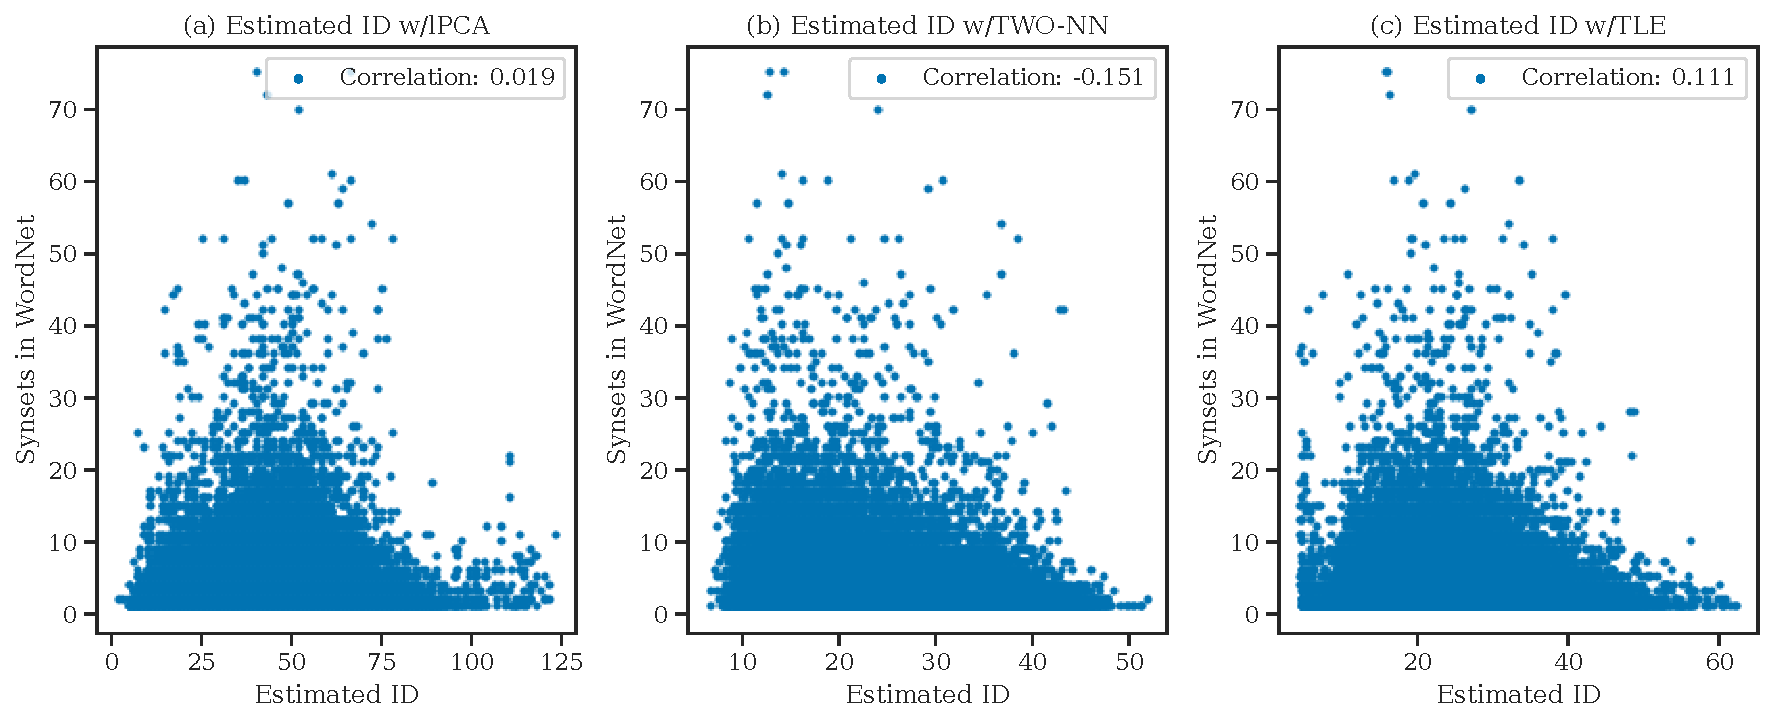
\includegraphics[width=\textwidth]{thesis/figures/intrinsic-dimension-estimation-vs-wordnet-synsets.pdf}
    \caption{Estimated IDs plotted against the number of word meanings, using LPCA, TWO-NN and TLE ID estimation algorithms.}
    \label{fig:intrinsic-dimension-estimation-vs-wordnet-synsets}
\end{figure}

We have now shown the relationship between estimated IDs and the number of word meanings. In the next section, we will create supervised models for predicting whether or not a word is polysemous. We will use multiple sets of hyperparameters and all ID estimation algorithms specified in \cref{sec:intrinsic-dimension-estimation}, as well the topological polysemy (\cref{sec:analysis-of-embeddings-topological-polysemy}) and Geometric Anomaly Detection (\cref{sec:analysis-of-embeddings-geometric-anomaly-detection}) algorithms.

\subsection{Supervised polysemy prediction}
\label{sec:analysis-of-embeddings-supervised-polysemy-prediction}
In this subsection, we will propose two supervised models to predict the number of word meanings. As we have seen in the previous subsections (\cref{sec:analysis-of-embeddings-topological-polysemy}, \cref{sec:analysis-of-embeddings-geometric-anomaly-detection} and \cref{sec:analysis-of-embeddings-intrinsic-dimension-estimation}), the number of word meanings seem to be more or less correlated with topological polysemy, Geometric Anomaly Detection (GAD) and intrinsic dimension (ID) estimation. For this reason, we will propose two supervised model using lasso regression (\cref{sec:lasso-regression}) and logistic regression (\cref{sec:logistic-regression}), incorporating the results from topological polysemy, GAD and ID estimation. We chose to use lasso regression because it has feature importance packed in the model. The feature importance part is important for us because we would like to try multiple configurations of hyperparameters for each algorithm used to create the training data. The logistic regression model is trained using $\ell_1$-penalty, allowing the model to perform feature importance. The lasso regression model tries to predict the number of word meanings, while the logistic regression model performs binary prediction of whether or not a word is polysemous. We also attempted to create a multi-class (e.g. one meaning, two meanings, etc.) model using multinomial logistic regression, but it became apparent that the problem was too hard and we decided not to follow up with those experiments. Furthermore, we denote the lasso regression model as \textit{WME-enwiki} (short for \textbf{W}ord \textbf{M}eaning \textbf{E}stimation-enwiki) and the logistic regression model as \textit{BWME-enwiki} (short for \textbf{B}inary \textbf{W}ord \textbf{M}eaning \textbf{E}stimation-enwiki). Next, we will describe the creation of training data used for both supervised models, before going into detail about the training and evaluation process.

To create the training data used in the WME- and BWME-enwiki models, we used the word embeddings from the SGNS-enwiki model. In particular, we used the word embeddings that have a WordNet entry, resulting in 144 412 words. We denote these word embeddings as the WordNet SGNS-enwiki word embeddings. The number of word meanings (i.e. the number of WordNet synsets) is used as labels $y$ for the WME-enwiki model. For the BWME-enwiki model, we used binary labels, i.e. $y=0$ if the word had exactly one word meaning, and $y=1$ if the word had two or more meanings.

To create the features of the training data, we first computed topological polysemy $\text{TPS}_n(w)$ of the WordNet SGNS-enwiki word embeddings. We computed $\text{TPS}_n(w)$ at for varying $n=10, 20, 30, \ldots, 250$ (step size of 10, leading to 25 values of $n$) and used them as features in the data. In addition to this, we computed the maximum, average and standard deviation of the birth values of the zero-degree persistence diagram computed by $\text{TPS}_n(w)$, leading to 3 additional features for each $\text{TPS}_n(w)$. In total, this resulted in 25 (values of $n$) $\times$ 4 = 100 features from topological polysemy.

Following, we applied GAD to the WordNet SGNS-enwiki word embeddings. To compute GAD, we used the $k$-nearest neighbour version, similar to the experiments of \cref{sec:analysis-of-embeddings-geometric-anomaly-detection}; we let the inner annulus radius equal the distance to the $s$-nearest neighbour and the outer annulus radius equal the distance to the $t$-nearest neighbour. Since we used the $k$-nearest neighbour version of GAD we were more in control of the computation time, because setting the radius manually can lead to large and difficult computations of the Vietoris–Rips complex, as some areas are denser than others. We show the different choices of $s$ and $t$ in \cref{table:supervised-polysemy-prediction-gad-configurations}, which leads to 23 different configurations of the inner and outer annulus $k$-nearest neighbours. We let the manifold dimension $k$ equal 2 for all words, even though the local intrinsic dimension for each word is likely higher than 2. This was done to make the GAD computation feasible within the computational resources at hand; we will revisit the manifold dimension choice when discussing future work in \cref{chap:conclusion-and-future-work}. For each of the $(s, t)$ configurations used to parameterize GAD, we created one feature for each GAD group (i.e. manifold, boundary and singular) as 3-dimensional one-hot encodings. For example, if a word is categorized as being on the manifold, then its value is equal to 1 and the rest are set to zero. In other words, we are left with 23 (configurations) $\times$ 3 (GAD groups) = 69 features from GAD. We also attempted to vectorize the persistence diagrams created by GAD using persistence images (\cref{sec:persistence-image}), but it quickly led to far too many features as we used each pixel in the images as a separate feature, and we were unable to train the WME- and BWME-enwiki models efficiently. We will revisit the use of persistence images when discussing future work in \cref{chap:conclusion-and-future-work}.
\begin{table}[H]
    \centering
    \begin{tabular}{@{}cc@{}}
    \toprule
    \multicolumn{1}{l}{Inner annulus, $s$-nearest neighbour} & \multicolumn{1}{l}{Outer annulus, $t$-nearest neighbour} \\
    \midrule
    \trcolor 25 & 250 \\
    25 & 500 \\
    \trcolor 25 & 750 \\
    25 & 1000 \\
    \midrule
    \trcolor 50 & 250 \\
    50 & 500 \\
    \trcolor 50 & 750 \\
    50 & 1000 \\
    \midrule
    \trcolor 100 & 1000 \\
    100 & 1250 \\
    \trcolor 100 & 1500 \\
    100 & 1750 \\
    \trcolor 100 & 2000 \\
    \midrule
    150 & 1000 \\
    \trcolor 150 & 1250 \\
    150 & 1500 \\
    \trcolor 150 & 1750 \\
    150 & 2000 \\
    \midrule
    \trcolor 200 & 1000 \\
    200 & 1250 \\
    \trcolor 200 & 1500 \\
    200 & 1750 \\
    \trcolor 200 & 2000 \\
    \bottomrule
    \end{tabular}
    \caption{Configurations of $s$ (inner annulus nearest neighbour) and $t$ (outer annulus nearest neighbour) for computing GAD of the WordNet SGNS-enwiki word embeddings.}
    \label{table:supervised-polysemy-prediction-gad-configurations}
\end{table}

Furthermore, we estimated the local ID of the WordNet SGNS-enwiki word embeddings using the ID estimation algorithms from \cref{sec:intrinsic-dimension-estimation}. More precisely, we used the LPCA (\cref{sec:id-estimation-lpca}), KNN (\cref{sec:id-estimation-knn}), TWO-NN (\cref{sec:id-estimation-twonn}), MLE (\cref{sec:id-estimation-mle}) and TLE (\cref{sec:id-estimation-tle}) algorithms. For each of the ID estimation algorithms, we used the $k$-nearest neighbours of each word to estimate their local IDs. We used the following values for $k$: 25, 50, 100, 150 and 200. The estimated local ID of each word is used as a feature in the training data, leading to 5 (algorithms) $\times$ 5 (hyperparameter sets) = 25 features from ID estimation. We used the \path{scikit-dimension} Python package \cite{scikitdimension2020} to estimate the local IDs.

In total, the training data had 100 (from topological polysemy) + 69 (from GAD) + 25 (from ID estimation) = 194 features. Following, we split the training data into three new distinct data sets (\cref{sec:train-val-test-splits}): training-, test- and SemEval test data sets. The new training data set consisted of 95\% random words of the original training data set, excluding the 100 SemEval-2010 Task 14 target words (\cref{sec:analysis-of-embeddings-topological-polysemy}). The test data set consisted of 5\% random words of the original training data set, excluding the 100 SemEval-2010 Task 14 target words. We will use the test data to evaluate the performance of the trained WME- and BWME-enwiki models. Furthermore, the SemEval test data set consisted of the 100 SemEval-2010 Task 14 target words and will be used to evaluate the performance using the WME-enwiki model. We emphasize that the training, test and SemEval test data sets do not have overlapping words, as we do not want to be training on words from the test data sets. The training data set consisted of 137 098 words, the test data set consisted of 7 216 words, and the SemEval test data set consisted of 98 words (as 2 of the words were out of the SGNS-enwiki vocabulary). For each data set, we transformed the features by removing the mean and scaling to unit variance, as we did not want the WME- and BWME-enwiki models to be affected by different means and variances across the features. For the SemEval test data set, we used the SemEval gold standard as the number of word meanings, while for the training and test data set we used the number of WordNet synsets as the number of word meanings.

Following, we trained the WME- and BWME-enwiki models using $k$-fold cross-validation (\cref{sec:cross-validation}). We found $k=20$ to work well with our data, meaning that we used 6855 random words for each fold in the cross-validation. For the WME-enwiki model, we cross-validated over 10000 values of $\lambda$, starting from $\lambda=0.0000001$ to $\lambda=0.01$. We found the most optimal value of $\lambda$ for the WME-enwiki model to be 0.0000291. For the BWME-enwiki model, we cross-validated over 10000 values of $\lambda$, starting from $\lambda=0.00001$ to $\lambda=0.01$. We found the most optimal value of $\lambda$ for the BWME-enwiki model to be 0.000692. To perform the cross-validation we used the \path{LassoCV} and \path{LogisticRegressionCV} classes from \path{scikit-learn} for the WME- and BWME-enwiki models, respectively. For the WME-enwiki model, we used the default scoring of the \path{LassoCV} class. On the other hand, for the BWME-enwiki model, our goal was to maximize the ability of the model to predict polysemous words accurately. As such, we used the sensitivity metric (\cref{sec:sensitivity}) to score the folds from the BWME-enwiki cross-validation. Furthermore, we show the results from training the WME-enwiki model in \cref{fig:wme-enwiki-correlation-result}, where we see a weak correlation between the predicted number of word meanings and the number of WordNet synsets for both the training and test data sets. In \cref{fig:wme-enwiki-correlation-result} (c), we see that the model is unable to predict the number of word meanings for the SemEval data set, which is not surprising, as we have trained using the number of WordNet synsets. We note, however, that we see clear trends in all plots of \cref{fig:wme-enwiki-correlation-result}.
\begin{figure}[H]
    \centering
    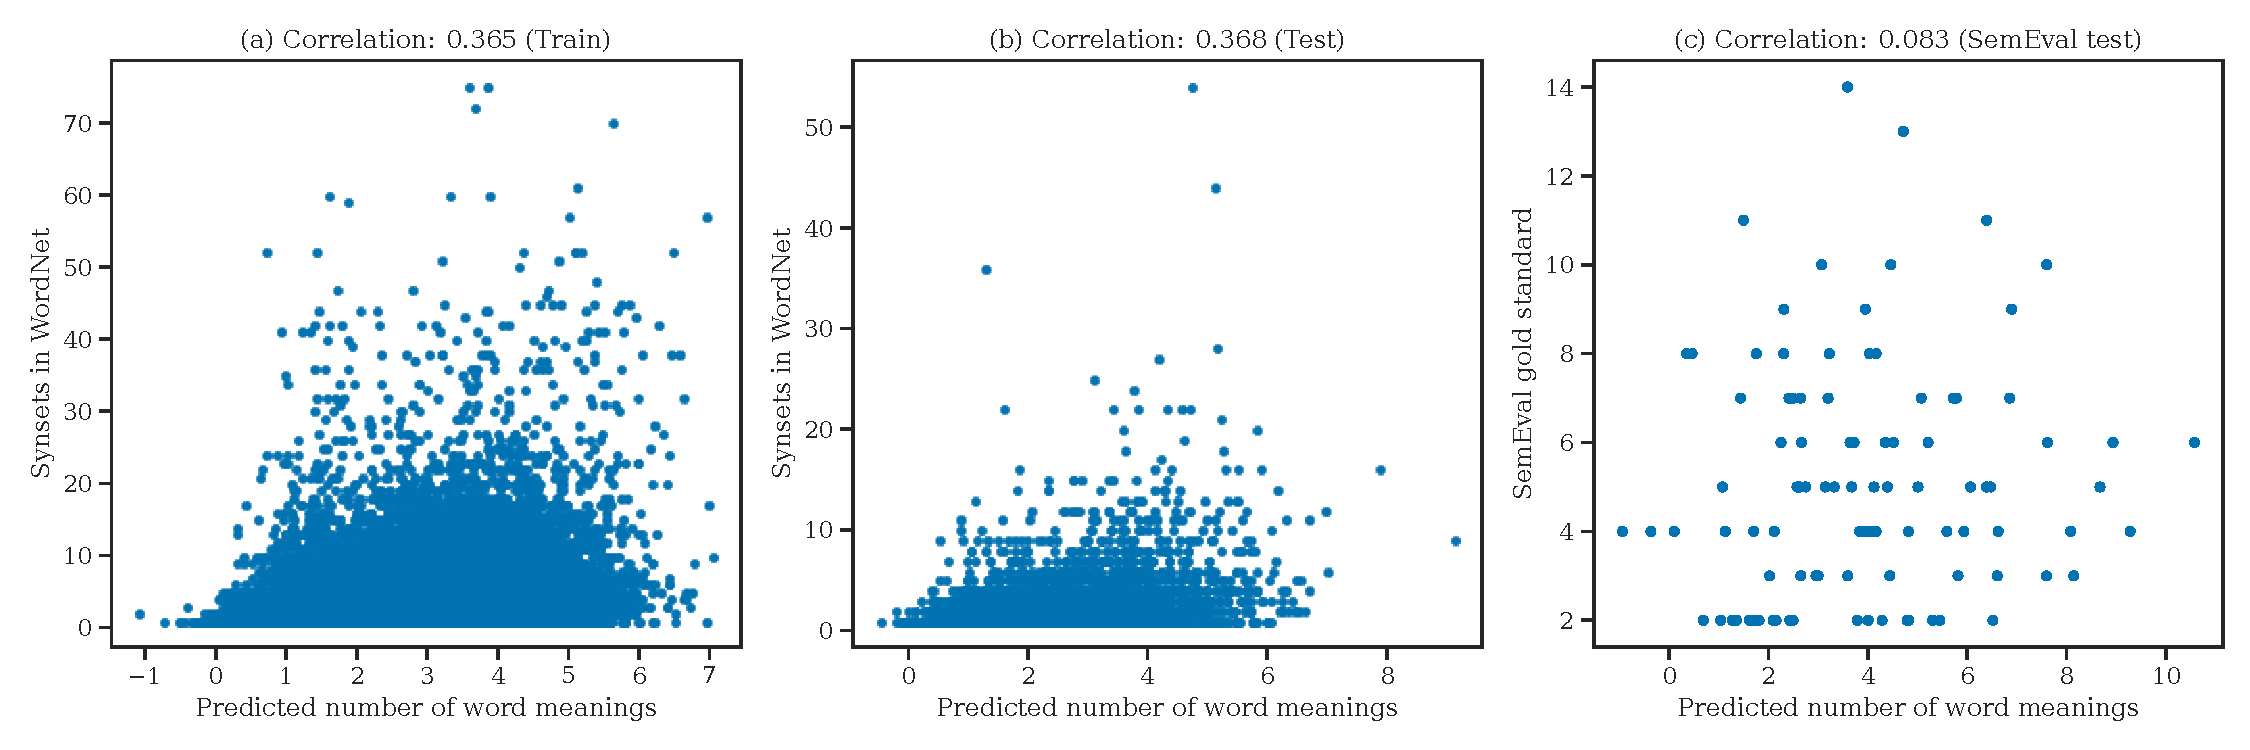
\includegraphics[width=\textwidth]{thesis/figures/wme-enwiki-correlation-result.pdf}
    \caption{The predicted number of word meanings plotted against the number of WordNet synsets and SemEval gold standard, using the WME-enwiki model.}
    \label{fig:wme-enwiki-correlation-result}
\end{figure}

By looking at the values of the feature coefficients of the WME-enwiki model, we saw how the model prioritized certain features over others. We show the top 10 most important features in \cref{fig:wme-enwiki-feature-importances}. In \cref{fig:wme-enwiki-feature-importances} we see that the features from topological polysemy are the most relevant for the model, for high values of $n$. The MLE and TLE intrinsic dimension estimators are also relatively relevant for high values of the $k$-nearest neighbour. The features from GAD are not in the top 10 most important features.
\begin{figure}[H]
    \centering
    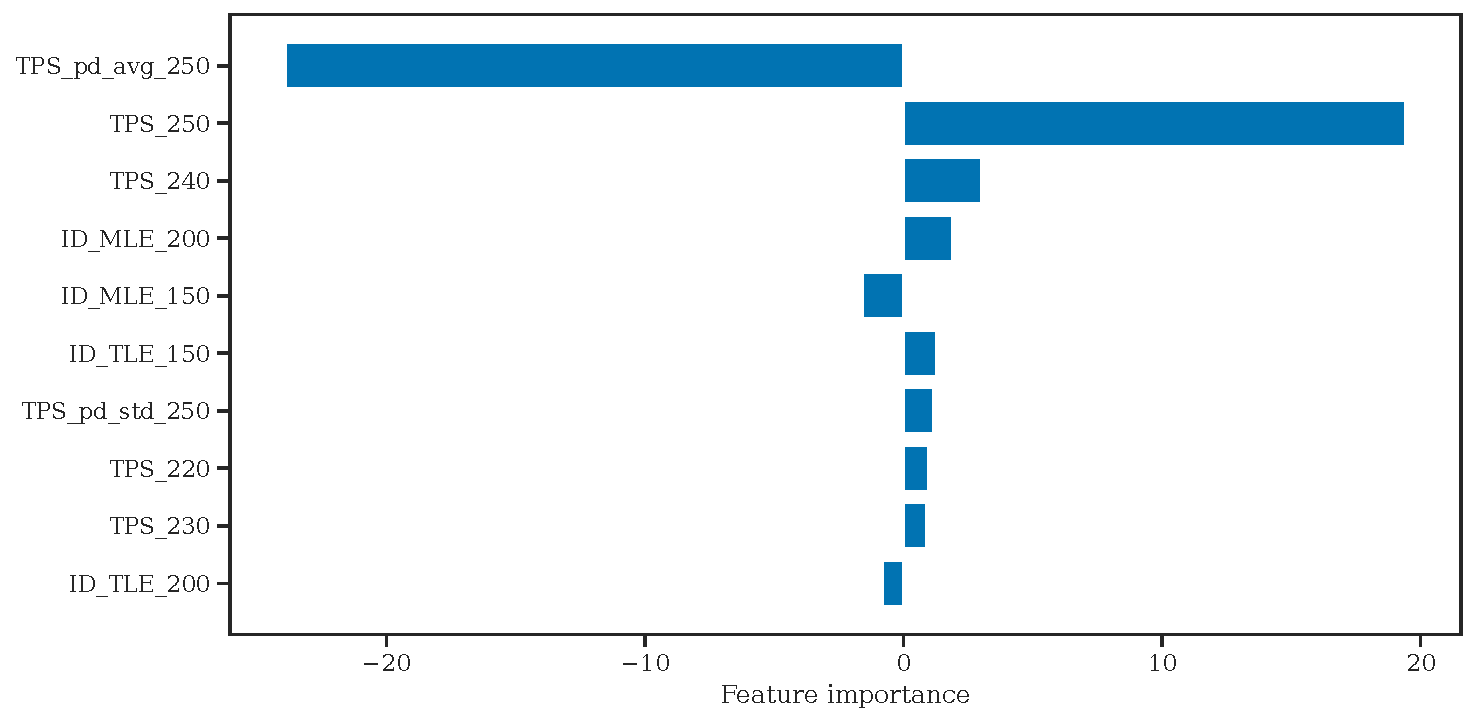
\includegraphics[width=\textwidth]{thesis/figures/wme-enwiki-top-10-feature-importances.pdf}
    \caption{Feature importances for the top 10 most important features of the WME-enwiki model.}
    \label{fig:wme-enwiki-feature-importances}
\end{figure}

To investigate the feature importances for the TPS, GAD and ID estimator features, we visualize its top 10 most important features in \cref{fig:wme-enwiki-feature-importances-tps-gad-estimated-ids}. In \cref{fig:wme-enwiki-feature-importances-tps-gad-estimated-ids}, we see that the $\text{TPS}_{250}$ features are especially relevant. From the GAD features in \cref{fig:wme-enwiki-feature-importances-tps-gad-estimated-ids} (b), we see that whether or not a word is classified as boundary or singular is important, while being classified as a manifold is not as relevant. Lastly, we see that the MLE and TLE ID estimator methods yield important features for various values of $n$. It should be noted, that the feature importance shown in \cref{fig:wme-enwiki-feature-importances-tps-gad-estimated-ids} (a) and (c) are more important than the features shown in \cref{fig:wme-enwiki-feature-importances-tps-gad-estimated-ids} (b), as noted by the x-axis scales.
\begin{figure}[H]
    \centering
    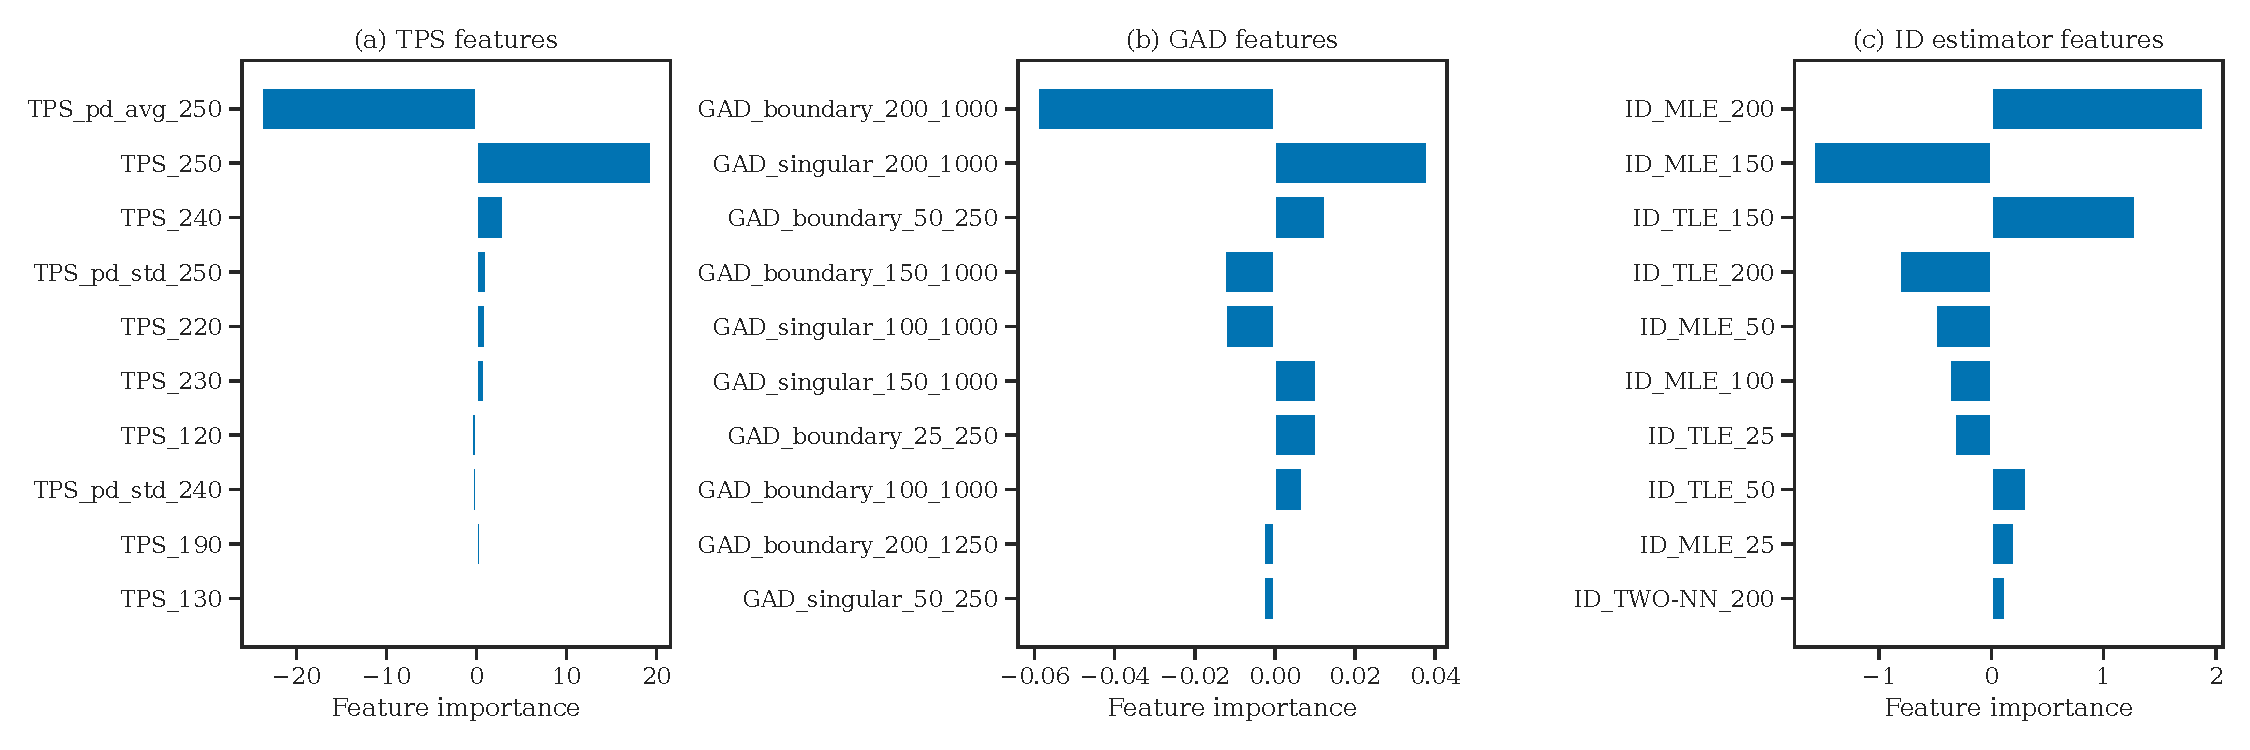
\includegraphics[width=\textwidth]{thesis/figures/wme-enwiki-top-10-feature-importances-tps-gad-estimated-ids.pdf}
    \caption{Feature importance of the top 10 TPS, GAD and ID estimator features, using the WME-enwiki model.}
    \label{fig:wme-enwiki-feature-importances-tps-gad-estimated-ids}
\end{figure}

From the training of the WME-enwiki model, the lasso set some of the features to zero, essentially removing them from the model. In particular, 48 of 194 features were set to zero, and most of them were various configurations of GAD which did not yield any interesting result (e.g. all words classified as boundary words). We have now looked at the results from training the WME-enwiki model, and in particular, looked at its performance for predicting the number of word meanings and which features were important to the model.

Next, we will look at the results from the training of the BWME-enwiki model. We show the results from the training of the BWME-enwiki model in \cref{fig:bwme-enwiki-confusion-matrices}, where we see the result of predicting the number of word meanings on the training and test data sets using confusion matrices (\cref{sec:confusion-matrix}). As we show in \cref{fig:bwme-enwiki-confusion-matrices}, we get a sensitivity of 0.393 on the train data sets, meaning that the model identifies 39.3\% of the polysemous words. The test sensitivity shows that the model identifies 39.4\% of all the unseen polysemous words. These results indicate that the model can not efficiently predict whether or not a word is polysemous, as we ideally would like the sensitivity on both the training and test sets to be at least 0.5 (or 50\%).
\begin{figure}[H]
    \centering
    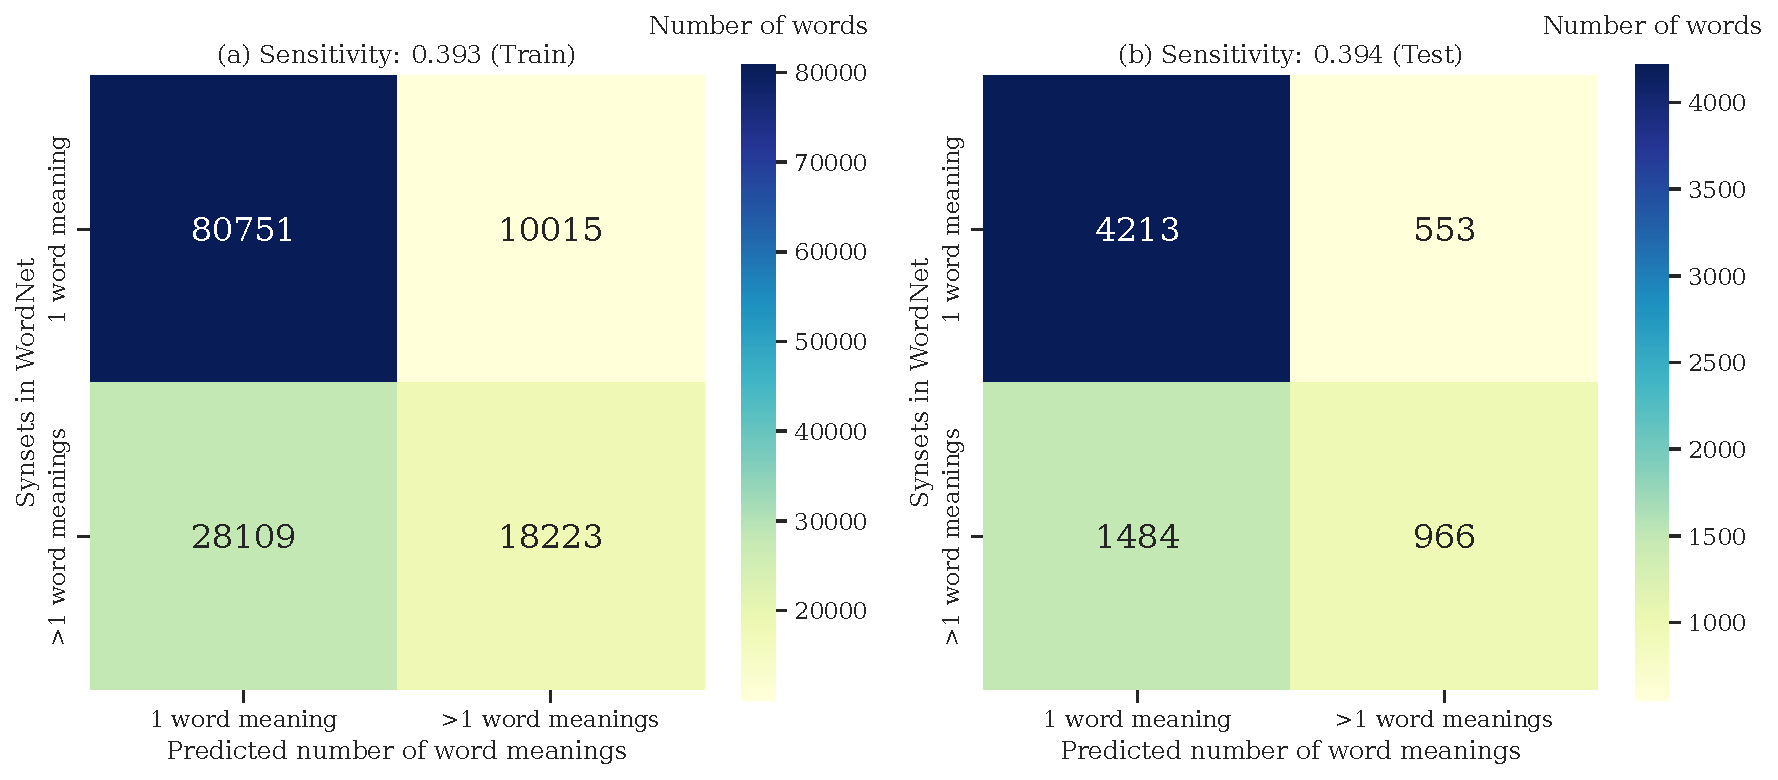
\includegraphics[width=\textwidth]{thesis/figures/bwme-enwiki-confusion-matrices.pdf}
    \caption{Confusion matrices for predicting the number of word meanings, using the BWME-enwiki model. The first confusion matrix (a) shows the result on the training data set, while the second confusion matrix (b) shows the result on the test data set.}
    \label{fig:bwme-enwiki-confusion-matrices}
\end{figure}

To deepen our understanding of which words the BWME-enwiki model has a harder time with, we looked at the misclassified polysemous test words. Of the 1484 words the BWME-enwiki model predicted to be monosemous, we report the top 10 most common misclassified test words, namely the following words: "time", "age", "returned", "Italian", "Chicago", "gold", "tower", "jones", "unable" and "opposition". From these words, we do not see any particular pattern. Furthermore, we visualize the words from the test data set in \cref{fig:bwme-enwiki-umap-misclassified-polysemous-words}, using a 2-dimensional UMAP embedding. In \cref{fig:bwme-enwiki-umap-misclassified-polysemous-words}, we emphasize the misclassified words, and we do not see any particular pattern here either, as the words are spread throughout the UMAP embedding.
\begin{figure}[H]
    \centering
    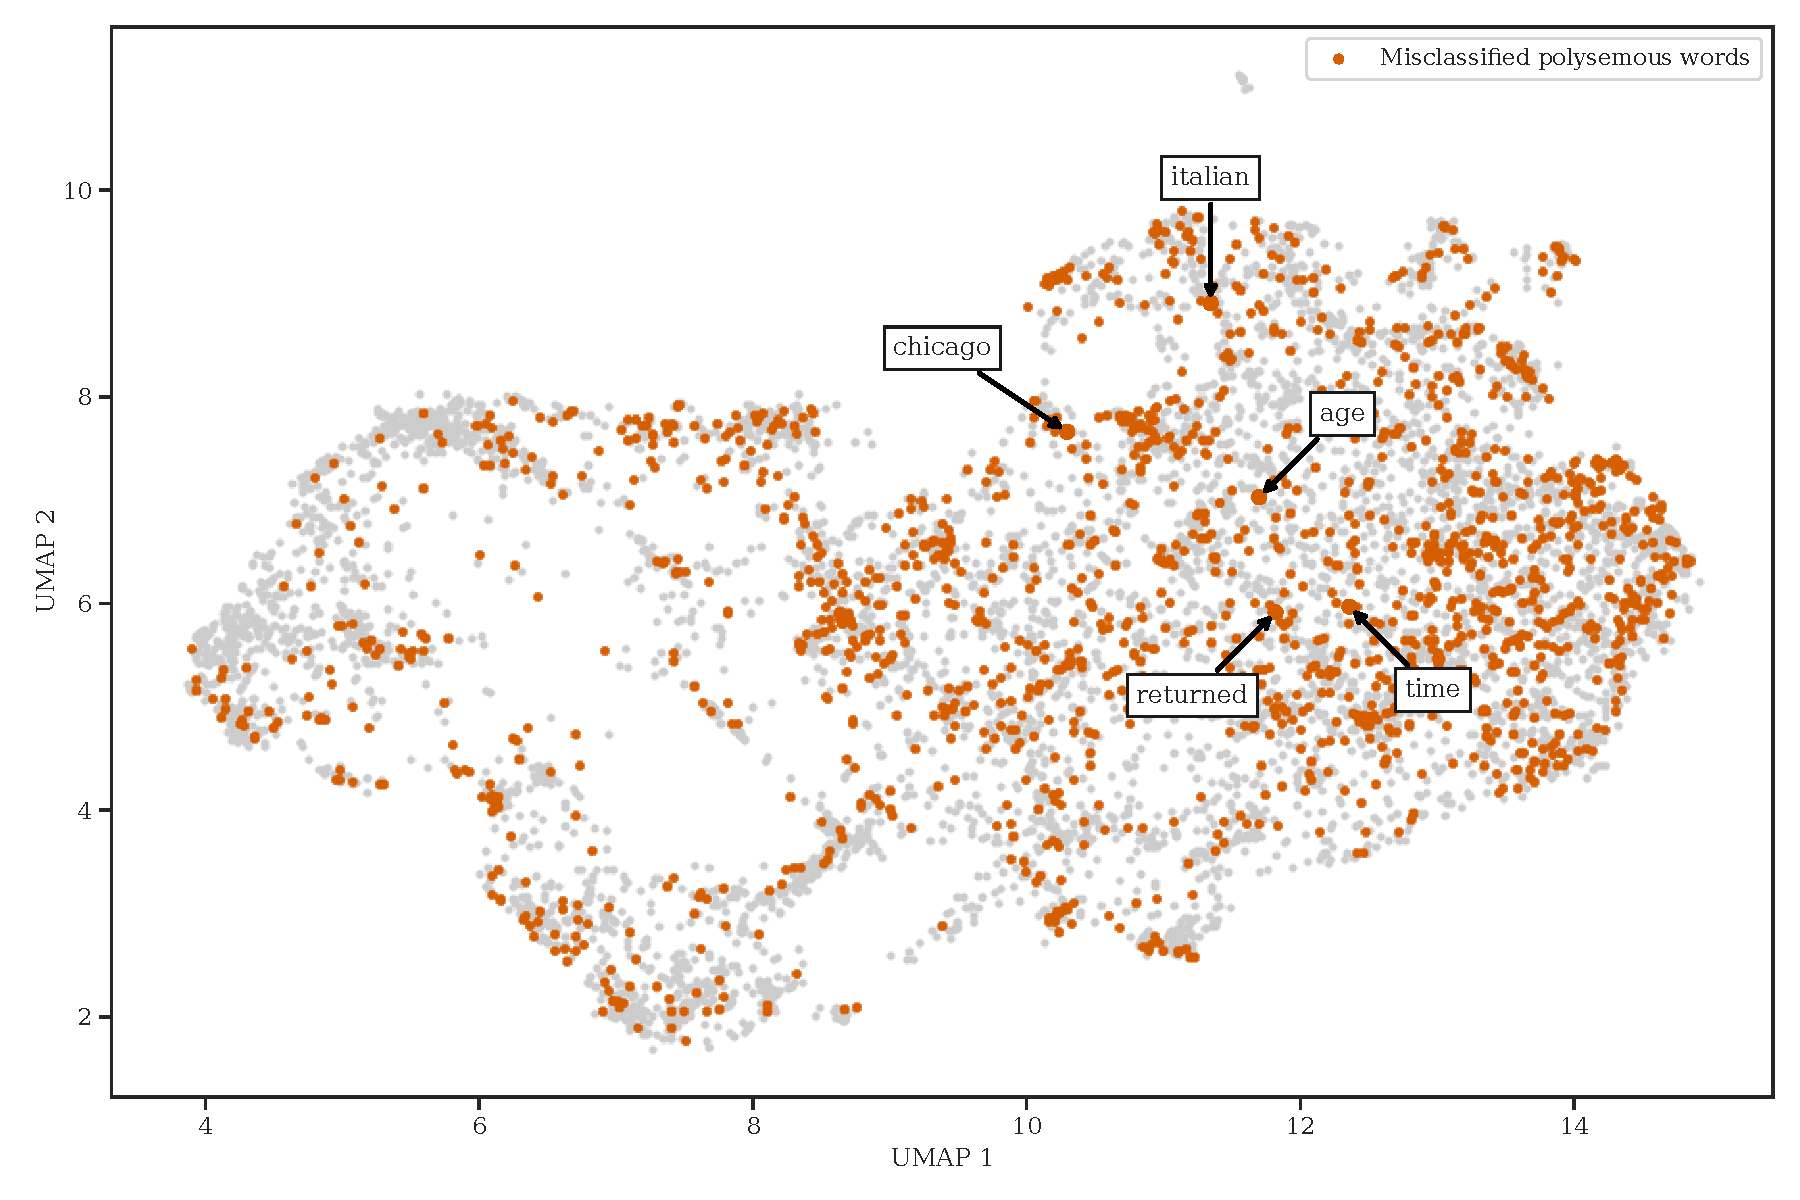
\includegraphics[width=\textwidth]{thesis/figures/bwme-enwiki-umap-misclassified-polysemous-words.pdf}
    \caption{2-dimensional UMAP embedding of the test data set evaluated on the BWME-enwiki model. We emphasize the misclassified polysemous words.}
    \label{fig:bwme-enwiki-umap-misclassified-polysemous-words}
\end{figure}

Next, we will investigate the feature importance in the BWME-enwiki model by looking at the coefficient values of the features. We show the top 10 most important features of the BWME-enwiki model in \cref{fig:bwme-enwiki-feature-importances}. In \cref{fig:bwme-enwiki-feature-importances}, we see a similar pattern to the top 10 features importances from the WME-enwiki model, namely that the TPS features (for varying $n$) are most important, followed by the features from the ID estimator models.
\begin{figure}[H]
    \centering
    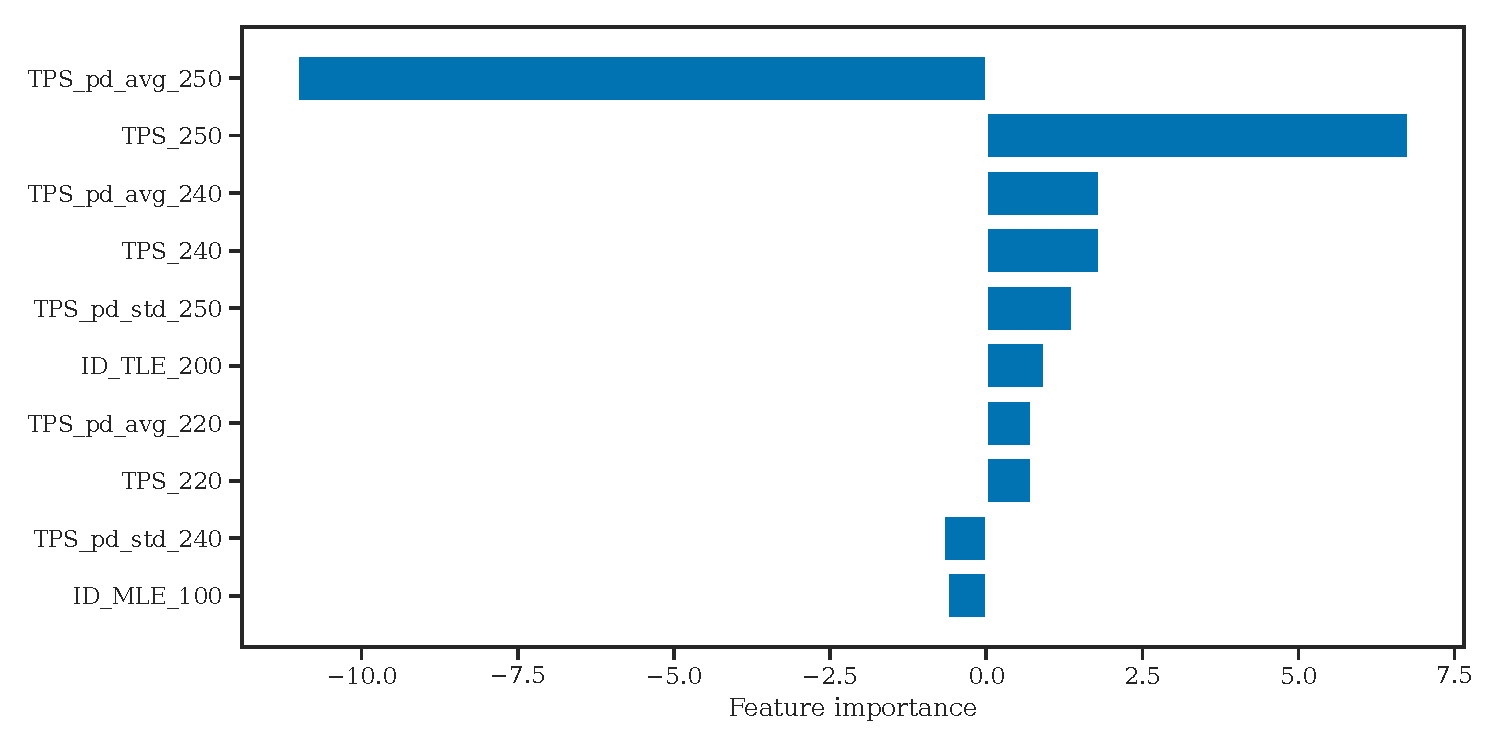
\includegraphics[width=\textwidth]{thesis/figures/bwme-enwiki-top-10-feature-importances.pdf}
    \caption{Feature importances for the top 10 most important features of the BWME-enwiki model.}
    \label{fig:bwme-enwiki-feature-importances}
\end{figure}

Furthermore, we look at the top 10 feature importances for the TPS, GAD and ID estimator features separately, as shown in \cref{fig:bwme-enwiki-feature-importances-tps-gad-estimated-ids}. In \cref{fig:bwme-enwiki-feature-importances-tps-gad-estimated-ids}, we see that the TPS features with high values of $n$ are generally more important than lower values. From the GAD features in \cref{fig:bwme-enwiki-feature-importances-tps-gad-estimated-ids} (b), we see a different situation to the top 10 features importances for GAD using the WME-enwiki model. In particular, we see that whether or not a point is categorized as singular is important for predicting whether or not a word is polysemous, and the rest of the GAD categories are less relevant. One interesting finding is that the GAD singular features importances were negative; we expected them to be positive, as it would make sense for them to be a positive contribution to whether or not a word is polysemous. Lastly, we see that the TLE and TLE ID estimator models yield important features for high neighbourhood values. Similar to the feature importances shown in \cref{fig:wme-enwiki-feature-importances-tps-gad-estimated-ids}, we note the fact that the feature importance shown in \cref{fig:bwme-enwiki-feature-importances-tps-gad-estimated-ids} (a) and (c) are more important than the features shown in \cref{fig:bwme-enwiki-feature-importances-tps-gad-estimated-ids} (b), as noted by the x-axis scales.
\begin{figure}[H]
    \centering
    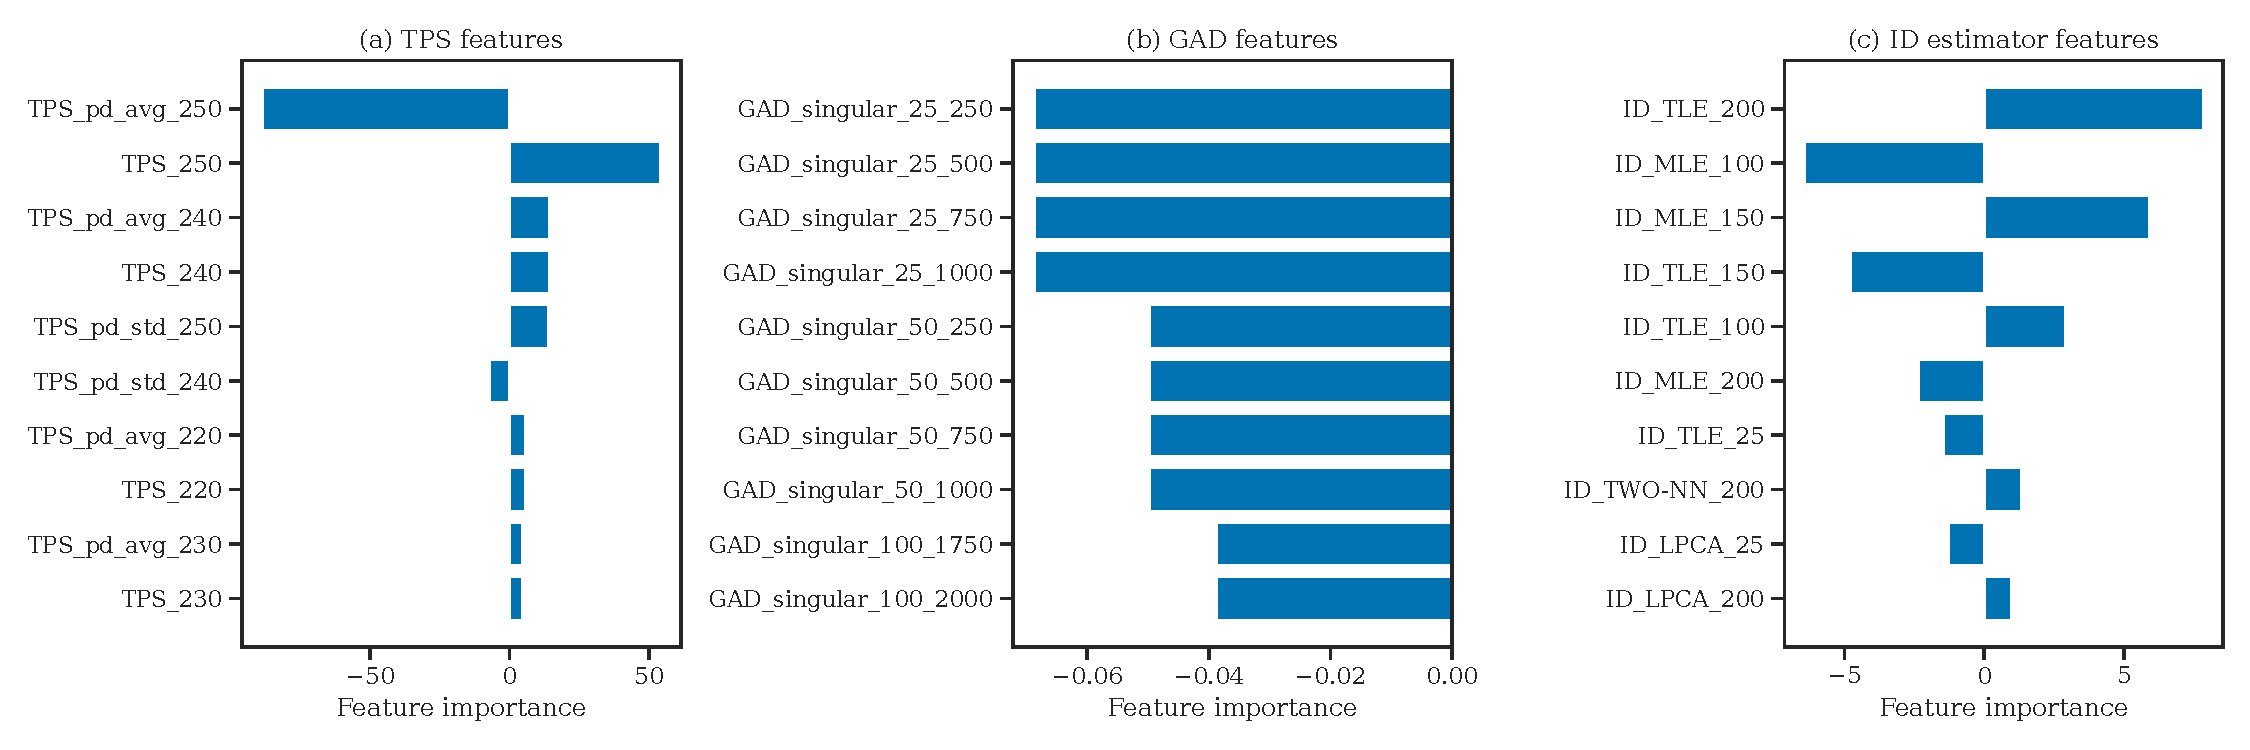
\includegraphics[width=\textwidth]{thesis/figures/bwme-enwiki-top-10-feature-importances-tps-gad-estimated-ids.pdf}
    \caption{Feature importance of the top 10 TPS, GAD and ID estimator features, using the BWME-enwiki model.}
    \label{fig:bwme-enwiki-feature-importances-tps-gad-estimated-ids}
\end{figure}

We have now explained how we trained and evaluated two supervised models for predicting the number of word meanings and whether or not a word is polysemous. Next, we will conclude the thesis and discuss ideas for future work.